%Chapter 2
\chapter{Overview of simulation and compressed air applications}
\label{Chap2}
\thispagestyle{empty}
\vspace{38em}
\hrulefill
\\
\enquote*{\textit{If I have seen further, it is by standing on the shoulders of giants.}} - Isaac Newton\\
\clearpage
\section{Introduction}
 This chapter will firstly provide relevant background on the operation and subcomponents of compressed air networks. A review of literature regarding compressed air energy interventions will then be performed. This review will summarise previous work to improve to improve the supply and demand efficiency of mining compressed air networks.
\par
The use of simulation in mining systems will then be reviewed. This section will summarise the usage of mathematical estimation and simulations tools in the mining industry. From the literature available simulation tools as well as simulation and verification procedures will be discussed.
\par
Finally simulation usage in compressed air systems will be discussed. The section will summarise the work, as well as the successes and shortfalls, that has already been performed with regard to simulation of large compressed air networks.
\section{Background on mining compressed air networks}
\subsection{Preamble}
Compressed air is used extensively in a mine in surface and underground operations. This section provides background regarding mining compressed air networks. The section firstly discusses the components that make up a mining compressed air system. The typical operation of the system is then examined. Finally the instrumentation that is typically installed in compresssed air networks is discussed
\subsection{Compressor air network components}
\subsubsection{Compressors}
 \footnotetext[1]{Abc oil refining, "How centrifugal compressors operate" [Online] \url{http://abcoilrefining.blogspot.co.za/2012/03/how-centrifugal-compressors-operate.html}, [Accessed 15 August 2017].}

Compressed air in mining is most commonly supplied by a centrifugal-type dynamic compressor \cite{Fouche2016Masters},\cite{Booysen2012Masters}.  These machines achieve compression as a result of the centrifugal force from the high-speed rotation of impellers in the air. The rotating impeller is  powered by a electric motor.
\par 
 Multi-stage impeller compressor designs, as shown in \cref{fig: Compressor diagram}\footnotemark[1], are used to obtain higher pressure ratios \cite{Fouche2016Masters}. The compression process is inefficient. Only about 5\% to 10\% of the input energy of the process is converted into energy that is used \cite{yang2009air}. 
\begin{figure}[h]
	\centering
	\fbox{\hspace{3.5cm}\begingroup
\makeatletter
\providecommand\color[2][]{%
	\GenericError{(gnuplot) \space\space\space\@spaces}{%
		Package color not loaded in conjunction with
		terminal option `colourtext'%
	}{See the gnuplot documentation for explanation.%
	}{Either use 'blacktext' in gnuplot or load the package
		color.sty in LaTeX.}%
	\renewcommand\color[2][]{}%
}%
\providecommand\includegraphics[2][]{%
	\GenericError{(gnuplot) \space\space\space\@spaces}{%
		Package graphicx or graphics not loaded%
	}{See the gnuplot documentation for explanation.%
	}{The gnuplot epslatex terminal needs graphicx.sty or graphics.sty.}%
	\renewcommand\includegraphics[2][]{}%
}%
\providecommand\rotatebox[2]{#2}%
\@ifundefined{ifGPcolor}{%
	\newif\ifGPcolor
	\GPcolortrue
}{}%
\@ifundefined{ifGPblacktext}{%
	\newif\ifGPblacktext
	\GPblacktextfalse
}{}%
% define a \g@addto@macro without @ in the name:
\let\gplgaddtomacro\g@addto@macro
% define empty templates for all commands taking text:
\gdef\gplbacktext{}%
\gdef\gplfronttext{}%
\makeatother
\ifGPblacktext
% no textcolor at all
\def\colorrgb#1{}%
\def\colorgray#1{}%
\else
% gray or color?
\ifGPcolor
\def\colorrgb#1{\color[rgb]{#1}}%
\def\colorgray#1{\color[gray]{#1}}%
\expandafter\def\csname LTw\endcsname{\color{white}}%
\expandafter\def\csname LTb\endcsname{\color{black}}%
\expandafter\def\csname LTa\endcsname{\color{black}}%
\expandafter\def\csname LT0\endcsname{\color[rgb]{1,0,0}}%
\expandafter\def\csname LT1\endcsname{\color[rgb]{0,1,0}}%
\expandafter\def\csname LT2\endcsname{\color[rgb]{0,0,1}}%
\expandafter\def\csname LT3\endcsname{\color[rgb]{1,0,1}}%
\expandafter\def\csname LT4\endcsname{\color[rgb]{0,1,1}}%
\expandafter\def\csname LT5\endcsname{\color[rgb]{1,1,0}}%
\expandafter\def\csname LT6\endcsname{\color[rgb]{0,0,0}}%
\expandafter\def\csname LT7\endcsname{\color[rgb]{1,0.3,0}}%
\expandafter\def\csname LT8\endcsname{\color[rgb]{0.5,0.5,0.5}}%
\else
% gray
\def\colorrgb#1{\color{black}}%
\def\colorgray#1{\color[gray]{#1}}%
\expandafter\def\csname LTw\endcsname{\color{white}}%
\expandafter\def\csname LTb\endcsname{\color{black}}%
\expandafter\def\csname LTa\endcsname{\color{black}}%
\expandafter\def\csname LT0\endcsname{\color{black}}%
\expandafter\def\csname LT1\endcsname{\color{black}}%
\expandafter\def\csname LT2\endcsname{\color{black}}%
\expandafter\def\csname LT3\endcsname{\color{black}}%
\expandafter\def\csname LT4\endcsname{\color{black}}%
\expandafter\def\csname LT5\endcsname{\color{black}}%
\expandafter\def\csname LT6\endcsname{\color{black}}%
\expandafter\def\csname LT7\endcsname{\color{black}}%
\expandafter\def\csname LT8\endcsname{\color{black}}%
\fi
\fi
\setlength{\unitlength}{0.0500bp}%
\ifx\gptboxheight\undefined%
\newlength{\gptboxheight}%
\newlength{\gptboxwidth}%
\newsavebox{\gptboxtext}%
\fi%
\setlength{\fboxrule}{0.5pt}%
\setlength{\fboxsep}{1pt}%
\begin{picture}(6000.00,5000.00)%
\put(0,250){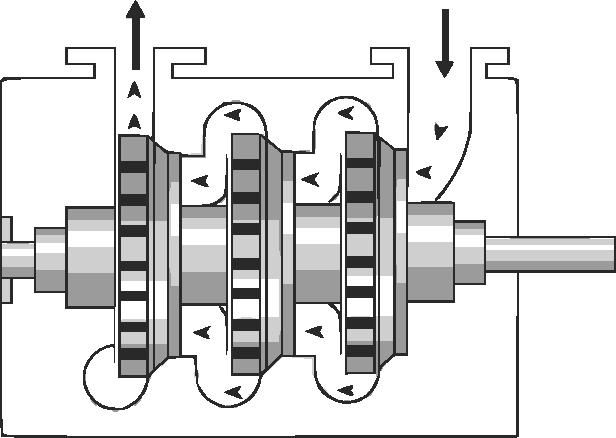
\includegraphics[width=0.65\textwidth]{Images/2/Compressor/Mcompressor}}%
      \put(4000,4750){\makebox(0,0)[l]{Suction}}%
      \put(1320,4750){{\makebox(0,0){\strut{}Discharge}}}%
      \put(1200,400){{\makebox(0,0){\strut{}Stage 3}}}%
      \put(2300,400){{\makebox(0,0){\strut{}Stage 2}}}%
      \put(3400,400){{\makebox(0,0){\strut{}Stage 1}}}%
      \put(5500,2400){{\makebox(0,0){\strut{}Rotor}}}%
    
\end{picture}%
\endgroup

\hspace{3cm}}
	\caption[A scematic of a multistage centrifugal compressor.]{A schematic of a multi-stage centrifugal compressor\protect \footnotemark[1].}
	\label{fig: Compressor diagram}
\end{figure}

\subsubsection{Pneumatic rock drills}
Drilling is mainly performed in the production areas or stopes of a mine. Drill machines are used to drill holes into the rock face. Once the holes have been drilled, explosives are then installed to break up the rock \cite{van2008development}.
\par
Compressed air is used to power pneumatic rock drills within a mine. Pneumatic rock drills run at an efficiency of 2\%. This is low when compared to alternative rock drills such as electric, oil electro-hydraulic and hydro-powered drills that convert energy at an efficiency of between 20-31\% \cite{fraser2008saving}, \cite{vanTonder2010Masters}. 
\subsubsection{Refuge bays}
Refuge bays are installed underground in deep level mines to provide safety to miners in the event of an emergency. Due safety regulations, most mines will utilise compressed air to deliver chilled air to the chamber \cite{brake1999criteria}. \cref{fig: Refuge Bay} shows an example of a compressed air inlet at an underground refuge bay. A muffler is installed to the end of the inlet air pipe to reduce noise.
\begin{figure}[h]
	\centering
	\fbox{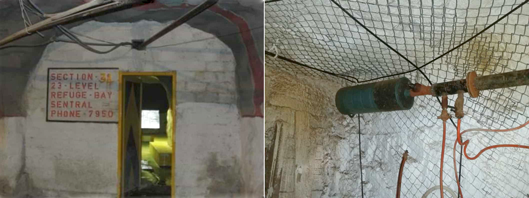
\includegraphics[width=\textwidth]{Images/1/refugebaysmall}}
	\caption{An example of compressed air inlet in an underground refuge bay chamber of a mine.}
	\label{fig: Refuge Bay}
\end{figure}
\par The provision of 1.42 $l/s$ of air per person at a pressure between 200 and 300 \gls{kpa} is required to provide oxygen and prevent any poisonousness gas entering the refuge \cite{brake1999criteria}.\par
Airflow in the refuge bays are controlled by a manual valve within the chamber. The manual vales are often misused by mine workers in order to cool the bay through decompression of the air. %[CitationNeeded]
\subsubsection{Processing plants}
Processing plants are constructed near gold and mines. They are used when extracting metal from the ore that is obtained from the mining operation. These plants use compressed air for various systems, processes and equipment. 
\par 
Processing plants often share compressed air network with mine to save costs\cite{Marais2012PhD}. The plants use relatively small amounts of air compared to mines. However, plant processes have pressure requirements that differ from the rest of the air network. If the plant air supply is not isolated from the shaft's air system, energy optimisations can be complicated. 
\subsubsection{Other compressed air users}
Due to the availability underground, compressed air is utilised for several other applications. These usages include, pneumatic loaders or rock shovels, pneumatic cylinders, dam sediment agitation, cooling and ventilation and many other applications. This vast variety of applications also leads to misuse of compressed air. This leads to inefficient operation.
\subsection{Operation schedule}
On a typical mine, various operations are scheduled different times of the day. Depending on the activity taking place, many mines will control the pressure to meet the requirements of the tasks \cite{Kriel2014Masters},\cite{Marais2012PhD}. \cref{fig: Mining schedule} shows the schedule and pressure requirement on a typical deep level mine.\par 
As shown in \cref{fig: Mining schedule}, the pressure requirement changes depending on the activity taking place. The drilling shift typically has the highest pressure requirement whilst blasting shift requires the lowest. Schedules and operation philosophies can differ between mines. Different operational schedules require alternative pressure requirement profiles.
\begin{figure}[h]
	\centering
	\fbox{% GNUPLOT: LaTeX picture with Postscript
\begingroup
  \makeatletter
  \providecommand\color[2][]{%
    \GenericError{(gnuplot) \space\space\space\@spaces}{%
      Package color not loaded in conjunction with
      terminal option `colourtext'%
    }{See the gnuplot documentation for explanation.%
    }{Either use 'blacktext' in gnuplot or load the package
      color.sty in LaTeX.}%
    \renewcommand\color[2][]{}%
  }%
  \providecommand\includegraphics[2][]{%
    \GenericError{(gnuplot) \space\space\space\@spaces}{%
      Package graphicx or graphics not loaded%
    }{See the gnuplot documentation for explanation.%
    }{The gnuplot epslatex terminal needs graphicx.sty or graphics.sty.}%
    \renewcommand\includegraphics[2][]{}%
  }%
  \providecommand\rotatebox[2]{#2}%
  \@ifundefined{ifGPcolor}{%
    \newif\ifGPcolor
    \GPcolortrue
  }{}%
  \@ifundefined{ifGPblacktext}{%
    \newif\ifGPblacktext
    \GPblacktextfalse
  }{}%
  % define a \g@addto@macro without @ in the name:
  \let\gplgaddtomacro\g@addto@macro
  % define empty templates for all commands taking text:
  \gdef\gplbacktext{}%
  \gdef\gplfronttext{}%
  \makeatother
  \ifGPblacktext
    % no textcolor at all
    \def\colorrgb#1{}%
    \def\colorgray#1{}%
  \else
    % gray or color?
    \ifGPcolor
      \def\colorrgb#1{\color[rgb]{#1}}%
      \def\colorgray#1{\color[gray]{#1}}%
      \expandafter\def\csname LTw\endcsname{\color{white}}%
      \expandafter\def\csname LTb\endcsname{\color{black}}%
      \expandafter\def\csname LTa\endcsname{\color{black}}%
      \expandafter\def\csname LT0\endcsname{\color[rgb]{1,0,0}}%
      \expandafter\def\csname LT1\endcsname{\color[rgb]{0,1,0}}%
      \expandafter\def\csname LT2\endcsname{\color[rgb]{0,0,1}}%
      \expandafter\def\csname LT3\endcsname{\color[rgb]{1,0,1}}%
      \expandafter\def\csname LT4\endcsname{\color[rgb]{0,1,1}}%
      \expandafter\def\csname LT5\endcsname{\color[rgb]{1,1,0}}%
      \expandafter\def\csname LT6\endcsname{\color[rgb]{0,0,0}}%
      \expandafter\def\csname LT7\endcsname{\color[rgb]{1,0.3,0}}%
      \expandafter\def\csname LT8\endcsname{\color[rgb]{0.5,0.5,0.5}}%
    \else
      % gray
      \def\colorrgb#1{\color{black}}%
      \def\colorgray#1{\color[gray]{#1}}%
      \expandafter\def\csname LTw\endcsname{\color{white}}%
      \expandafter\def\csname LTb\endcsname{\color{black}}%
      \expandafter\def\csname LTa\endcsname{\color{black}}%
      \expandafter\def\csname LT0\endcsname{\color{black}}%
      \expandafter\def\csname LT1\endcsname{\color{black}}%
      \expandafter\def\csname LT2\endcsname{\color{black}}%
      \expandafter\def\csname LT3\endcsname{\color{black}}%
      \expandafter\def\csname LT4\endcsname{\color{black}}%
      \expandafter\def\csname LT5\endcsname{\color{black}}%
      \expandafter\def\csname LT6\endcsname{\color{black}}%
      \expandafter\def\csname LT7\endcsname{\color{black}}%
      \expandafter\def\csname LT8\endcsname{\color{black}}%
    \fi
  \fi
    \setlength{\unitlength}{0.0500bp}%
    \ifx\gptboxheight\undefined%
      \newlength{\gptboxheight}%
      \newlength{\gptboxwidth}%
      \newsavebox{\gptboxtext}%
    \fi%
    \setlength{\fboxrule}{0.5pt}%
    \setlength{\fboxsep}{1pt}%
\begin{picture}(9360.00,4032.00)%
    \gplgaddtomacro\gplbacktext{%
      \colorrgb{0.00,0.00,0.00}%
      \put(814,1364){\makebox(0,0)[r]{\strut{}$400$}}%
      \colorrgb{0.00,0.00,0.00}%
      \put(814,1615){\makebox(0,0)[r]{\strut{}$420$}}%
      \colorrgb{0.00,0.00,0.00}%
      \put(814,1866){\makebox(0,0)[r]{\strut{}$440$}}%
      \colorrgb{0.00,0.00,0.00}%
      \put(814,2117){\makebox(0,0)[r]{\strut{}$460$}}%
      \colorrgb{0.00,0.00,0.00}%
      \put(814,2368){\makebox(0,0)[r]{\strut{}$480$}}%
      \colorrgb{0.00,0.00,0.00}%
      \put(814,2618){\makebox(0,0)[r]{\strut{}$500$}}%
      \colorrgb{0.00,0.00,0.00}%
      \put(814,2869){\makebox(0,0)[r]{\strut{}$520$}}%
      \colorrgb{0.00,0.00,0.00}%
      \put(814,3120){\makebox(0,0)[r]{\strut{}$540$}}%
      \colorrgb{0.00,0.00,0.00}%
      \put(814,3371){\makebox(0,0)[r]{\strut{}$560$}}%
      \colorrgb{0.00,0.00,0.00}%
      \put(946,1232){\rotatebox{-270}{\makebox(0,0)[r]{\strut{}00:00}}}%
      \colorrgb{0.00,0.00,0.00}%
      \put(1295,1232){\rotatebox{-270}{\makebox(0,0)[r]{\strut{}01:00}}}%
      \colorrgb{0.00,0.00,0.00}%
      \put(1643,1232){\rotatebox{-270}{\makebox(0,0)[r]{\strut{}02:00}}}%
      \colorrgb{0.00,0.00,0.00}%
      \put(1992,1232){\rotatebox{-270}{\makebox(0,0)[r]{\strut{}03:00}}}%
      \colorrgb{0.00,0.00,0.00}%
      \put(2340,1232){\rotatebox{-270}{\makebox(0,0)[r]{\strut{}04:00}}}%
      \colorrgb{0.00,0.00,0.00}%
      \put(2689,1232){\rotatebox{-270}{\makebox(0,0)[r]{\strut{}05:00}}}%
      \colorrgb{0.00,0.00,0.00}%
      \put(3037,1232){\rotatebox{-270}{\makebox(0,0)[r]{\strut{}06:00}}}%
      \colorrgb{0.00,0.00,0.00}%
      \put(3386,1232){\rotatebox{-270}{\makebox(0,0)[r]{\strut{}07:00}}}%
      \colorrgb{0.00,0.00,0.00}%
      \put(3734,1232){\rotatebox{-270}{\makebox(0,0)[r]{\strut{}08:00}}}%
      \colorrgb{0.00,0.00,0.00}%
      \put(4083,1232){\rotatebox{-270}{\makebox(0,0)[r]{\strut{}09:00}}}%
      \colorrgb{0.00,0.00,0.00}%
      \put(4431,1232){\rotatebox{-270}{\makebox(0,0)[r]{\strut{}10:00}}}%
      \colorrgb{0.00,0.00,0.00}%
      \put(4780,1232){\rotatebox{-270}{\makebox(0,0)[r]{\strut{}11:00}}}%
      \colorrgb{0.00,0.00,0.00}%
      \put(5128,1232){\rotatebox{-270}{\makebox(0,0)[r]{\strut{}12:00}}}%
      \colorrgb{0.00,0.00,0.00}%
      \put(5477,1232){\rotatebox{-270}{\makebox(0,0)[r]{\strut{}13:00}}}%
      \colorrgb{0.00,0.00,0.00}%
      \put(5825,1232){\rotatebox{-270}{\makebox(0,0)[r]{\strut{}14:00}}}%
      \colorrgb{0.00,0.00,0.00}%
      \put(6174,1232){\rotatebox{-270}{\makebox(0,0)[r]{\strut{}15:00}}}%
      \colorrgb{0.00,0.00,0.00}%
      \put(6522,1232){\rotatebox{-270}{\makebox(0,0)[r]{\strut{}16:00}}}%
      \colorrgb{0.00,0.00,0.00}%
      \put(6871,1232){\rotatebox{-270}{\makebox(0,0)[r]{\strut{}17:00}}}%
      \colorrgb{0.00,0.00,0.00}%
      \put(7219,1232){\rotatebox{-270}{\makebox(0,0)[r]{\strut{}18:00}}}%
      \colorrgb{0.00,0.00,0.00}%
      \put(7568,1232){\rotatebox{-270}{\makebox(0,0)[r]{\strut{}19:00}}}%
      \colorrgb{0.00,0.00,0.00}%
      \put(7916,1232){\rotatebox{-270}{\makebox(0,0)[r]{\strut{}20:00}}}%
      \colorrgb{0.00,0.00,0.00}%
      \put(8265,1232){\rotatebox{-270}{\makebox(0,0)[r]{\strut{}21:00}}}%
      \colorrgb{0.00,0.00,0.00}%
      \put(8613,1232){\rotatebox{-270}{\makebox(0,0)[r]{\strut{}22:00}}}%
      \colorrgb{0.00,0.00,0.00}%
      \put(8962,1232){\rotatebox{-270}{\makebox(0,0)[r]{\strut{}23:00}}}%
    }%
    \gplgaddtomacro\gplfronttext{%
      \csname LTb\endcsname%
      \put(176,2367){\rotatebox{-270}{\makebox(0,0){\strut{}kPa}}}%
      \put(4954,374){\makebox(0,0){\strut{}Time of day}}%
      \put(4954,3701){\makebox(0,0){\strut{}Typical mining schedule and pressure requirement}}%
      \csname LTb\endcsname%
      \put(6242,173){\makebox(0,0)[r]{\strut{}Pressure requirement (kPa)}}%
      \csname LTb\endcsname%
      \put(1817,2368){\rotatebox{-270}{\makebox(0,0){\strut{}\shortstack{Sweeping and \\ cleaning}}}}%
      \put(3037,2368){\rotatebox{-270}{\makebox(0,0){\strut{}\shortstack{Workers travel to \\ working areas}}}}%
      \put(4605,2368){\makebox(0,0){\strut{}\shortstack{Drilling}}}%
      \put(6174,2368){\rotatebox{-270}{\makebox(0,0){\strut{}\shortstack{Explosive charge \\ up}}}}%
      \put(7394,2368){\makebox(0,0){\strut{}\shortstack{Blasting}}}%
      \put(8613,2368){\rotatebox{-270}{\makebox(0,0){\strut{}\shortstack{Sweeping and \\ cleaning}}}}%
    }%
    \gplbacktext
    \put(0,0){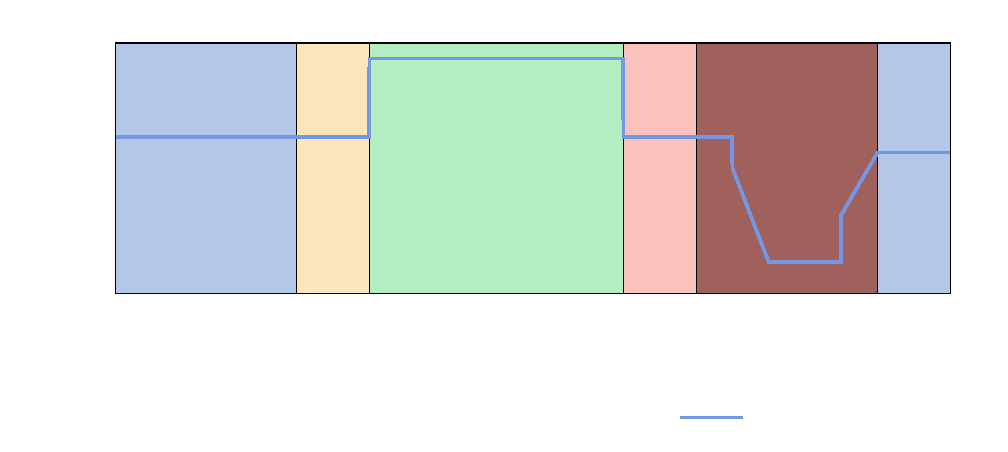
\includegraphics{Graphs/1/MiningSchedule/MiningSchedule}}%
    \gplfronttext
  \end{picture}%
\endgroup
}
	\caption[A typical operation schedule of a deep level mine.]{The typical operation schedule of a deep level mine \cite{Kriel2014Masters}.}
	\label{fig: Mining schedule}
\end{figure}
\subsection{Instrumentation}
For large industrial systems, thorough instrumentation is necessary to monitor performance and equipment conditions throughout the system. In a mining compressed air network, instrumentation is installed to monitor flows, pressures, temperatures and other process parameters. Electrical instrumentation is also installed for sensing currents, power factors, voltages and power. Parameters that are often measured include valves input/output pressures and flows, valve and guide vain positions and air condition metrics are usually measured with instrumentation.	
\par
A \gls{scada} system is used to monitor and control processes throughout the mine. The instrumentation and \gls{scada} are connected on a communication network.
This communication between the underground \glspl{plc} and surface \gls{scada} is achieved using a substantial fibre optic network\cite{schroeder2009energy}. The \gls{scada} centralises instrumentation data from \glspl{plc} and instrumentation in  the mine. The \gls{scada} is also used to control machines and control instrumentation by transmitting control signals over the network.  
\subsection{Summary}
In this section various sub-components of compressed air networks were discussed. These sub-components included compressors, processing plants as well as underground air users. The daily  process scheduling and the effect on compressed air requirements were then discussed. Finally the typical instrumentation found in a mining compressed air system was summarised.
\section{Review of compressed air energy interventions in industry}
	\subsection{Preamble}
		Compressed air improvement can be obtained through intervention in either the supply or demand processes of a compressed air system \cite{Kriel2014Masters}. Improvements in supply is achieved by increasing the efficiency of compressed air supply. Examples of these types of intervention include \gls{dcs}, compressor relocation, repairs and maintenance, etc. 
		\par
		Due to the size of mining compressed air networks, there is often a larger scope for improvement in air demand. Improving the demand is achieved by optimising air flow consumers, reducing leaks, etc.
		\par
	 	 This section will review compressed air supply and demand interventions that have improved energy or operation efficiency the mining industry. From the literature, successes and shortcomings in studies will be discussed and analysed with regard to this study.
	 	
	\subsection{Strategies to improve compressed air supply}

	%	\subsubsection{Compressor efficiency improvements}
	%	- literature regarding 
		\subsubsection{Optimising compressor control}
		Compressors types and numbers can differ widely from mining compressed air systems. Compressor selection is crucial in these systems to match the correct compressors with the requirements of the system \cite{marais2010expert}.
		\par 
		In a study by Booysen \cite{Booysen2012Masters} found that many mines control compressors using fixed target pressure points that are much higher than required. In one system, compressor controllers were set to target 650 \glssymbol{kpa} to ensure pressure underground did not fall below 500 \glssymbol{kpa}. Use of high set-points can lead to excessive wasteful blow-off air flow when the pressure exceeds maximum points.
		\par
		 \cite{booysen2009optimising} showed through dynamic pressure set-point control\footnote{Matching the supplied pressure with the specific required air demand.} and optimal compressor selection, energy savings can be achieved. In a case study, an average power reduction of 1.07 MW was achieved. The lead to an estimated energy cost saving of R3M.
		\par 
	 	Optimising control of compressors to match the demand of the system can be complicated. \glspl{vsd} and guide-vain are used to control the capacity of the system. More effective power reductions can be achieved through the use of \gls{vsd} control. Running compressors at part load reduces efficiency. From literature, it has been shown electric motors will typical use 60-80\% of there rated power when running at less than 50\% load \cite{Saidur2010}.
		%\subsubsection{Air storage}
		%- booysen 1.22
		%\subsubsection{Dynamic compressor selection}
		%- van Tonder PHD
		%- van heerden 
		\subsubsection{Reconfiguring compressed air networks}
			A number of old mining compressed air systems  have not been adequately maintained and improved. Often they cannot sufficiently supply air to meet the demand or air is provided from non optimal sources. In a study by Bredenkamp \cite{Bredenkamp2013Masters}, reconfiguring of the air network was investigated to improve these systems.
			\par  
			In the study, Bredenkamp investigated interconnecting the compressed air systems of two mining shafts and relocating of a compressor. This strategy lead to an average power reduction of 1.7 MW and an estimated annual energy cost saving of R8.9M at the time.
			%\par 
			%*** \textit{Discussion of Bredenkamp} shortcomings and successes ***
			
	\subsection{Strategies to reduce compressed air demand}
	Reducing the airflow demand is achieved by reducing air unnecessary airflow such as leaks, optimising the operating pressure to match the demand\footnotemark[2] and by improving the efficiency of air usage or replacing equipment with non-pneumatic alternatives \cite{Snyman2011Masters}.
		 \footnotetext[2]{This is achieved by identifying the minimum required operating pressure for all times of the day as illustrated in \cref{fig: Mining schedule}}
		 \subsubsection{Leakage detection}	 
		 Air leaks are a major inefficiency in mining compressed air systems. Improving leaks is relatively easier method to  reduce air demand and improve the efficiency of the system \cite{van2011sustaining}. Air leaks occur as a result of open pipes, fissure and breaks. Losses depend on the size of the leak and pressure in the network. \cref{fig: Leak losses} shows the theoretical airflow of through a pipe orifice as a function of leakage area and pressure\footnotemark[1]. \cite{van2011sustaining} showed that the system power consumption linearly increases with the amount of air leakage. Therefore, energy savings can be achieved through either reducing pressure or detecting and fixing leaks.
		 \begin{figure}[h]
		 	\centering
		 	\fbox{\hspace{2cm}% GNUPLOT: LaTeX picture with Postscript
\begingroup
  \makeatletter
  \providecommand\color[2][]{%
    \GenericError{(gnuplot) \space\space\space\@spaces}{%
      Package color not loaded in conjunction with
      terminal option `colourtext'%
    }{See the gnuplot documentation for explanation.%
    }{Either use 'blacktext' in gnuplot or load the package
      color.sty in LaTeX.}%
    \renewcommand\color[2][]{}%
  }%
  \providecommand\includegraphics[2][]{%
    \GenericError{(gnuplot) \space\space\space\@spaces}{%
      Package graphicx or graphics not loaded%
    }{See the gnuplot documentation for explanation.%
    }{The gnuplot epslatex terminal needs graphicx.sty or graphics.sty.}%
    \renewcommand\includegraphics[2][]{}%
  }%
  \providecommand\rotatebox[2]{#2}%
  \@ifundefined{ifGPcolor}{%
    \newif\ifGPcolor
    \GPcolortrue
  }{}%
  \@ifundefined{ifGPblacktext}{%
    \newif\ifGPblacktext
    \GPblacktextfalse
  }{}%
  % define a \g@addto@macro without @ in the name:
  \let\gplgaddtomacro\g@addto@macro
  % define empty templates for all commands taking text:
  \gdef\gplbacktext{}%
  \gdef\gplfronttext{}%
  \makeatother
  \ifGPblacktext
    % no textcolor at all
    \def\colorrgb#1{}%
    \def\colorgray#1{}%
  \else
    % gray or color?
    \ifGPcolor
      \def\colorrgb#1{\color[rgb]{#1}}%
      \def\colorgray#1{\color[gray]{#1}}%
      \expandafter\def\csname LTw\endcsname{\color{white}}%
      \expandafter\def\csname LTb\endcsname{\color{black}}%
      \expandafter\def\csname LTa\endcsname{\color{black}}%
      \expandafter\def\csname LT0\endcsname{\color[rgb]{1,0,0}}%
      \expandafter\def\csname LT1\endcsname{\color[rgb]{0,1,0}}%
      \expandafter\def\csname LT2\endcsname{\color[rgb]{0,0,1}}%
      \expandafter\def\csname LT3\endcsname{\color[rgb]{1,0,1}}%
      \expandafter\def\csname LT4\endcsname{\color[rgb]{0,1,1}}%
      \expandafter\def\csname LT5\endcsname{\color[rgb]{1,1,0}}%
      \expandafter\def\csname LT6\endcsname{\color[rgb]{0,0,0}}%
      \expandafter\def\csname LT7\endcsname{\color[rgb]{1,0.3,0}}%
      \expandafter\def\csname LT8\endcsname{\color[rgb]{0.5,0.5,0.5}}%
    \else
      % gray
      \def\colorrgb#1{\color{black}}%
      \def\colorgray#1{\color[gray]{#1}}%
      \expandafter\def\csname LTw\endcsname{\color{white}}%
      \expandafter\def\csname LTb\endcsname{\color{black}}%
      \expandafter\def\csname LTa\endcsname{\color{black}}%
      \expandafter\def\csname LT0\endcsname{\color{black}}%
      \expandafter\def\csname LT1\endcsname{\color{black}}%
      \expandafter\def\csname LT2\endcsname{\color{black}}%
      \expandafter\def\csname LT3\endcsname{\color{black}}%
      \expandafter\def\csname LT4\endcsname{\color{black}}%
      \expandafter\def\csname LT5\endcsname{\color{black}}%
      \expandafter\def\csname LT6\endcsname{\color{black}}%
      \expandafter\def\csname LT7\endcsname{\color{black}}%
      \expandafter\def\csname LT8\endcsname{\color{black}}%
    \fi
  \fi
    \setlength{\unitlength}{0.0500bp}%
    \ifx\gptboxheight\undefined%
      \newlength{\gptboxheight}%
      \newlength{\gptboxwidth}%
      \newsavebox{\gptboxtext}%
    \fi%
    \setlength{\fboxrule}{0.5pt}%
    \setlength{\fboxsep}{1pt}%
\begin{picture}(7200.00,5040.00)%
    \gplgaddtomacro\gplbacktext{%
      \colorrgb{0.00,0.00,0.00}%
      \put(1727,1050){\makebox(0,0){\strut{}$0.025$}}%
      \colorrgb{0.00,0.00,0.00}%
      \put(2545,900){\makebox(0,0){\strut{}$0.05$}}%
      \colorrgb{0.00,0.00,0.00}%
      \put(3363,750){\makebox(0,0){\strut{}$0.075$}}%
      \colorrgb{0.00,0.00,0.00}%
      \put(4180,600){\makebox(0,0){\strut{}$0.1$}}%
      \colorrgb{0.00,0.00,0.00}%
      \put(4500,755){\makebox(0,0){\strut{}$200$}}%
      \colorrgb{0.00,0.00,0.00}%
      \put(4810,927){\makebox(0,0){\strut{}$300$}}%
      \colorrgb{0.00,0.00,0.00}%
      \put(5120,1098){\makebox(0,0){\strut{}$400$}}%
      \colorrgb{0.00,0.00,0.00}%
      \put(5430,1270){\makebox(0,0){\strut{}$500$}}%
      \colorrgb{0.00,0.00,0.00}%
      \put(5750,1441){\makebox(0,0){\strut{}$600$}}%
      \colorrgb{0.00,0.00,0.00}%
      \put(6100,1613){\makebox(0,0){\strut{}$700$}}%
      \colorrgb{0.00,0.00,0.00}%
      \put(6370,1784){\makebox(0,0){\strut{}$800$}}%
      \colorrgb{0.00,0.00,0.00}%
      \put(920,2070){\makebox(0,0)[r]{\strut{}$0$}}%
      \colorrgb{0.00,0.00,0.00}%
      \put(920,2527){\makebox(0,0)[r]{\strut{}$1.5$}}%
      \colorrgb{0.00,0.00,0.00}%
      \put(920,2984){\makebox(0,0)[r]{\strut{}$3$}}%
      \colorrgb{0.00,0.00,0.00}%
      \put(920,3441){\makebox(0,0)[r]{\strut{}$4.5$}}%
    }%
    \gplgaddtomacro\gplfronttext{%
      \csname LTb\endcsname%
      \put(2198,750){\rotatebox{-9}{\makebox(0,0){\strut{}Area ($m^2$)}}}%
      \put(6029,1156){\rotatebox{30}{\makebox(0,0){\strut{}Pressure (kPa)}}}%
      \put(250,2755){\rotatebox{-270}{\makebox(0,0){\strut{}Flow (kg/s)}}}%
    }%
    \gplbacktext
    \put(0,0){\fbox{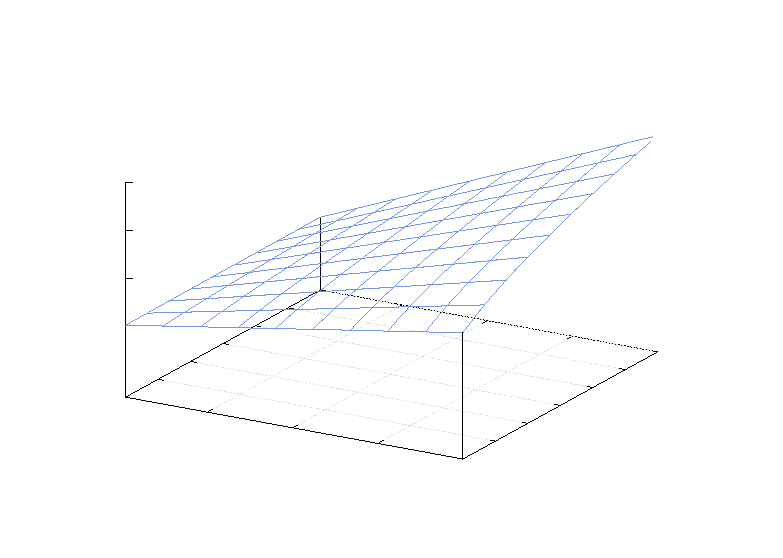
\includegraphics[trim=0 0 0.1cm 0, clip]{Graphs/2/Leak2/Leak2}}}%
    \gplfronttext
  \end{picture}%
\endgroup
\hspace{2cm}}
		 	\caption[The leakage flow as a function of inlet pressure and leakage area]{ The leakage flow as a function of inlet pressure and leakage area\protect\footnotemark[3].}
		 	\label{fig: Leak losses}
		 \end{figure}
	 \footnotetext[3]{efunda, "Orifice Flowmeter Calculator." [Online] \url{http://www.efunda.com/formulae/fluids/calc_orifice_flowmeter.cfm}, [Accessed 18 October 2016].}
	 \par 
		 Leaks are often not easily detected through visual methods. In industry, a number of techniques are employed to detect air leaks. Pascoe \cite{Pascoe2016Masters} and van Tonder \cite{vanTonder2010Masters} summarised these techniques as follows:
		 \begin{itemize}
		 	\item Audible detection (Walk and report)
		 	\item Ultrasonic detection
		 	\item Intelligent systems\footnote{Leakage detection by using strategically placed measurement equipment and smart computer systems.}
		 	\item "Pigging"\footnote{The use of a device, "pig", within the pipe to perform inspections.}
		 	\item Soap water/visible dyes 
		 \end{itemize}
	 	 These methods are time and resource intensive and many mines do not actively employ dedicated leakage detection and repair teams. Marais \textit{et al} \cite{marais2009increased} investigated streamlining the leakage detection and repair process to increase energy savings through the use of \gls{calds}. The system was developed to allow centralised mobile leakage reporting. Usage of \gls{calds} in mines resulted in an increased leak detection rate. One mine reporting 24 leaks in a single month. It was noted in the study that there difficulty quantifying the actual energy savings of the leakage repairs due to other intervention occurring simultaneously.	
		 
		 \subsubsection{Underground control valves optimisation}
		 Many mines utilise automated valves at critical locations or levels in the compressed air network. These valves control the pressure, restricting airflow from that point in the air network. Restricting airflow reduces losses resultant from network inefficiencies and leaks.
		 \par 
		 Kleingeld and Marais \cite{kleingeld2010high} found that optimising control valve control on mining levels can conservatively lead to between 20\% on mines where no control valves are installed. For systems that already have some form of network control, between 10 and 15\% savings can conservatively be achieved.
		 \par 
		 From literature, the advantage of control valve optimisation is the significant savings that can be achieved with relatively short set-up up time. Savings can be achieved incrementally with each control valve installation. Studies did not look at accurate estimations of savings or the shaft pressure improvements that result from control valve optimisation.	 
		\subsubsection{Improving pneumatic rock drill efficiency}
		 Pneumatic rock drills are on of the largest air consumers in a mine. However Pneumatic drilling systems convert energy very inefficiently. Replacing pneumatic drills with more efficient alternatives such as hydraulic or pneumatic drills would lead to large energy savings \cite{Pascoe2016Masters}.  Alternatively improving the efficiency of pneumatic drilling can have a significant energy impact on the system, without the cost and safety concerns of alternative drilling technologies.
		 \par 
		 In a study by  Bester \textit{et al.} \cite{bester2013effect} looking at the effect of compressed air pressure on energy demand. Bester showed that between 2002 and 2013 compressed air and energy consumption per tonne of ore produced had steadily increased. This is illustrated  in \cref{fig: Compressed energy and air flow per ton}. 
		  \par
		 The increase of air consumption per \gls{t} was a result of reduced air pressure at the mining areas. This caused a drop in the drilling rate, leading to higher air consumption. Pressure measurements as low as 300 \gls{kpa} were recorded in these areas. Before 2002 the drilling pressure at the mining section (stopes), was maintained above 500 \gls{kpa} at most mines. 
		 \par 
		 \begin{figure}[h]
		 	\centering
		 	% GNUPLOT: LaTeX picture with Postscript
\begingroup
  \makeatletter
  \providecommand\color[2][]{%
    \GenericError{(gnuplot) \space\space\space\@spaces}{%
      Package color not loaded in conjunction with
      terminal option `colourtext'%
    }{See the gnuplot documentation for explanation.%
    }{Either use 'blacktext' in gnuplot or load the package
      color.sty in LaTeX.}%
    \renewcommand\color[2][]{}%
  }%
  \providecommand\includegraphics[2][]{%
    \GenericError{(gnuplot) \space\space\space\@spaces}{%
      Package graphicx or graphics not loaded%
    }{See the gnuplot documentation for explanation.%
    }{The gnuplot epslatex terminal needs graphicx.sty or graphics.sty.}%
    \renewcommand\includegraphics[2][]{}%
  }%
  \providecommand\rotatebox[2]{#2}%
  \@ifundefined{ifGPcolor}{%
    \newif\ifGPcolor
    \GPcolortrue
  }{}%
  \@ifundefined{ifGPblacktext}{%
    \newif\ifGPblacktext
    \GPblacktextfalse
  }{}%
  % define a \g@addto@macro without @ in the name:
  \let\gplgaddtomacro\g@addto@macro
  % define empty templates for all commands taking text:
  \gdef\gplbacktext{}%
  \gdef\gplfronttext{}%
  \makeatother
  \ifGPblacktext
    % no textcolor at all
    \def\colorrgb#1{}%
    \def\colorgray#1{}%
  \else
    % gray or color?
    \ifGPcolor
      \def\colorrgb#1{\color[rgb]{#1}}%
      \def\colorgray#1{\color[gray]{#1}}%
      \expandafter\def\csname LTw\endcsname{\color{white}}%
      \expandafter\def\csname LTb\endcsname{\color{black}}%
      \expandafter\def\csname LTa\endcsname{\color{black}}%
      \expandafter\def\csname LT0\endcsname{\color[rgb]{1,0,0}}%
      \expandafter\def\csname LT1\endcsname{\color[rgb]{0,1,0}}%
      \expandafter\def\csname LT2\endcsname{\color[rgb]{0,0,1}}%
      \expandafter\def\csname LT3\endcsname{\color[rgb]{1,0,1}}%
      \expandafter\def\csname LT4\endcsname{\color[rgb]{0,1,1}}%
      \expandafter\def\csname LT5\endcsname{\color[rgb]{1,1,0}}%
      \expandafter\def\csname LT6\endcsname{\color[rgb]{0,0,0}}%
      \expandafter\def\csname LT7\endcsname{\color[rgb]{1,0.3,0}}%
      \expandafter\def\csname LT8\endcsname{\color[rgb]{0.5,0.5,0.5}}%
    \else
      % gray
      \def\colorrgb#1{\color{black}}%
      \def\colorgray#1{\color[gray]{#1}}%
      \expandafter\def\csname LTw\endcsname{\color{white}}%
      \expandafter\def\csname LTb\endcsname{\color{black}}%
      \expandafter\def\csname LTa\endcsname{\color{black}}%
      \expandafter\def\csname LT0\endcsname{\color{black}}%
      \expandafter\def\csname LT1\endcsname{\color{black}}%
      \expandafter\def\csname LT2\endcsname{\color{black}}%
      \expandafter\def\csname LT3\endcsname{\color{black}}%
      \expandafter\def\csname LT4\endcsname{\color{black}}%
      \expandafter\def\csname LT5\endcsname{\color{black}}%
      \expandafter\def\csname LT6\endcsname{\color{black}}%
      \expandafter\def\csname LT7\endcsname{\color{black}}%
      \expandafter\def\csname LT8\endcsname{\color{black}}%
    \fi
  \fi
    \setlength{\unitlength}{0.0500bp}%
    \ifx\gptboxheight\undefined%
      \newlength{\gptboxheight}%
      \newlength{\gptboxwidth}%
      \newsavebox{\gptboxtext}%
    \fi%
    \setlength{\fboxrule}{0.5pt}%
    \setlength{\fboxsep}{1pt}%
\begin{picture}(9360.00,4032.00)%
    \gplgaddtomacro\gplbacktext{%
      \colorrgb{0.42,0.42,0.42}%
      \put(682,924){\makebox(0,0)[r]{\strut{}$0$}}%
      \colorrgb{0.42,0.42,0.42}%
      \put(682,1230){\makebox(0,0)[r]{\strut{}$5$}}%
      \colorrgb{0.42,0.42,0.42}%
      \put(682,1536){\makebox(0,0)[r]{\strut{}$10$}}%
      \colorrgb{0.42,0.42,0.42}%
      \put(682,1842){\makebox(0,0)[r]{\strut{}$15$}}%
      \colorrgb{0.42,0.42,0.42}%
      \put(682,2148){\makebox(0,0)[r]{\strut{}$20$}}%
      \colorrgb{0.42,0.42,0.42}%
      \put(682,2453){\makebox(0,0)[r]{\strut{}$25$}}%
      \colorrgb{0.42,0.42,0.42}%
      \put(682,2759){\makebox(0,0)[r]{\strut{}$30$}}%
      \colorrgb{0.42,0.42,0.42}%
      \put(682,3065){\makebox(0,0)[r]{\strut{}$35$}}%
      \colorrgb{0.42,0.42,0.42}%
      \put(682,3371){\makebox(0,0)[r]{\strut{}$40$}}%
      \colorrgb{0.42,0.42,0.42}%
      \put(814,704){\makebox(0,0){\strut{}$2002$}}%
      \colorrgb{0.42,0.42,0.42}%
      \put(2025,704){\makebox(0,0){\strut{}$2004$}}%
      \colorrgb{0.42,0.42,0.42}%
      \put(3237,704){\makebox(0,0){\strut{}$2006$}}%
      \colorrgb{0.42,0.42,0.42}%
      \put(4448,704){\makebox(0,0){\strut{}$2008$}}%
      \colorrgb{0.42,0.42,0.42}%
      \put(5659,704){\makebox(0,0){\strut{}$2010$}}%
      \colorrgb{0.42,0.42,0.42}%
      \put(6871,704){\makebox(0,0){\strut{}$2012$}}%
      \colorrgb{0.42,0.42,0.42}%
      \put(8082,704){\makebox(0,0){\strut{}$2014$}}%
      \colorrgb{0.42,0.42,0.42}%
      \put(8214,924){\makebox(0,0)[l]{\strut{}$0$}}%
      \colorrgb{0.42,0.42,0.42}%
      \put(8214,1230){\makebox(0,0)[l]{\strut{}$50$}}%
      \colorrgb{0.42,0.42,0.42}%
      \put(8214,1536){\makebox(0,0)[l]{\strut{}$100$}}%
      \colorrgb{0.42,0.42,0.42}%
      \put(8214,1842){\makebox(0,0)[l]{\strut{}$150$}}%
      \colorrgb{0.42,0.42,0.42}%
      \put(8214,2148){\makebox(0,0)[l]{\strut{}$200$}}%
      \colorrgb{0.42,0.42,0.42}%
      \put(8214,2453){\makebox(0,0)[l]{\strut{}$250$}}%
      \colorrgb{0.42,0.42,0.42}%
      \put(8214,2759){\makebox(0,0)[l]{\strut{}$300$}}%
      \colorrgb{0.42,0.42,0.42}%
      \put(8214,3065){\makebox(0,0)[l]{\strut{}$350$}}%
      \colorrgb{0.42,0.42,0.42}%
      \put(8214,3371){\makebox(0,0)[l]{\strut{}$400$}}%
    }%
    \gplgaddtomacro\gplfronttext{%
      \csname LTb\endcsname%
      \put(176,2147){\rotatebox{-270}{\makebox(0,0){\strut{}kWh/t}}}%
      \put(8851,2147){\rotatebox{-270}{\makebox(0,0){\strut{}$m^3$/t}}}%
      \put(4448,374){\makebox(0,0){\strut{}Year}}%
      \put(4448,3701){\makebox(0,0){\strut{}Compressed air energy and Volume consumed per ton}}%
      \csname LTb\endcsname%
      \put(3593,173){\makebox(0,0)[r]{\strut{}Energy per Ton (kWh/t)}}%
      \csname LTb\endcsname%
      \put(7352,173){\makebox(0,0)[r]{\strut{}Volume per Ton ($m^3$/t)}}%
    }%
    \gplbacktext
    \put(0,0){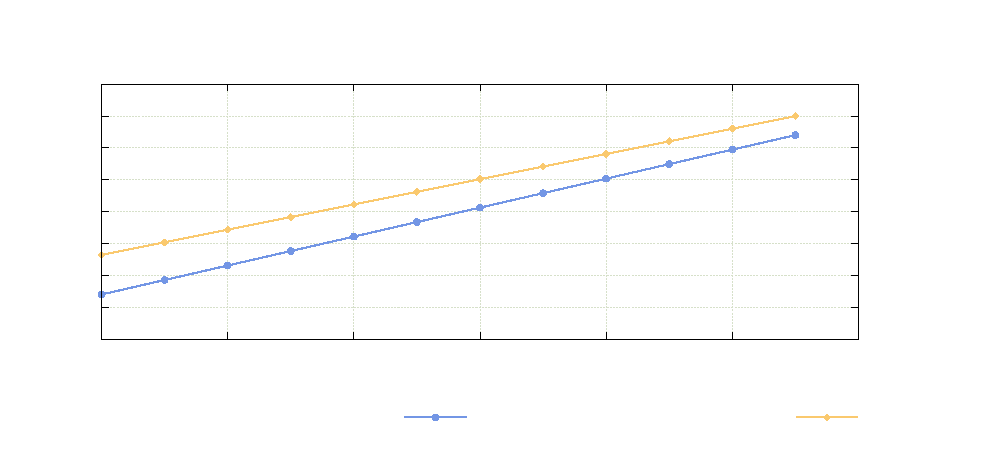
\includegraphics{Graphs/1/EVperT/EVperT}}%
    \gplfronttext
  \end{picture}%
\endgroup

		 	\caption[The Compressed air energy and flow consumed per T of ore produced.]{The Compressed air energy and flow consumed per T of ore produced. Adopted from Bester \textit{et al.}\cite{bester2013effect}.}
		 	\label{fig: Compressed energy and air flow per ton}
		 \end{figure}
		 From literature, it is shown that lowering the pressure reduces the efficiency and drill rate of rock drilling, leading to higher air consumption. Interventions that reduce systemic air losses or optimise supply can increase the pressure operating pressure. Increased pressure, during the drilling shift, may add more value than the energy cost savings that can be achieved at a lower pressure.
	\subsection{Summary}
	This section reviewed previous studies that had achieved energy improvements in compressed air. The literature was divided into studies that focussed on improving the supply of compressed air and those that optimised the compressed air demand.
	\par
	Compressed air supply interventions included optimising compressor control and reconfiguring compressor networks. On the demand side, studies that investigated reducing leaks, optimising underground valve control and improving rock drill efficiency were discussed.
\section{Use of simulations to identify improvements in mining systems}
	\subsection{Preamble}
	The value of simulation in the mining industry has been largely shown through its usage in \gls{dsm} initiatives. Simulation and estimation procedures have been widely applied to identify and pre-emptively quantify the effect of energy interventions strategies for water reticulation cooling, compressed air and ventilation systems.
	\par
	 The purpose of this section is to summarise and discuss the work that has been done in with regard to estimation and simulation of mining systems. This section will also discuss simulation development procedures and verification methodologies that have been applied in literature.
	
	\subsection{Estimating energy savings on mining systems }
	Estimation has been a vital tool in literature to obtain the potential energy impact that can be achieved from interventions on a mining system. Before new tools allowed for quick development of simplified simulation models, estimation techniques were frequently used to determine the feasibility of energy interventions. The shortcomings of the estimation approach is that they typically rely on simplified system models that lead to high prediction error, limit the complexity of scenarios and input/output variables.
		\par 
	Snyman \cite{Snyman2011Masters} used mathematical estimation to determine the expected power savings from initiatives on mining compressed air systems.  Due to uncertainty in the estimations, \cite{Snyman2011Masters} predicted results were provided as a range between conservative and best-case estimates. The actual achieved energy impact would fall between these estimations. Snyman's model only estimated the average energy impact and could not provide a resultant power profile or other output variables such as pressure.
		 	
		\subsubsection{Benchmark modelling}
		 Cilliers \cite{Cilliers2015PHD} developed \enquote{best practice models} using the \gls{cols} benchmarking method. These models provide an energy benchmark that can be used to identify the scope for energy improvement on mining systems. An example of a benchmark model for a mining compressed air system is shown in \cref{eq: COLS}. The model can be used to estimate optimal energy required as a function of the quantity of ore mined(T) and the depth of the mine (Z). \cite{Cilliers2015PHD} also developed benchmark models for mine cooling, water reticulation and ventilation systems.
		\begin{figure}[h!]
			\centering
			\fbox{\hspace{2cm}% GNUPLOT: LaTeX picture with Postscript
\begingroup
  \makeatletter
  \providecommand\color[2][]{%
    \GenericError{(gnuplot) \space\space\space\@spaces}{%
      Package color not loaded in conjunction with
      terminal option `colourtext'%
    }{See the gnuplot documentation for explanation.%
    }{Either use 'blacktext' in gnuplot or load the package
      color.sty in LaTeX.}%
    \renewcommand\color[2][]{}%
  }%
  \providecommand\includegraphics[2][]{%
    \GenericError{(gnuplot) \space\space\space\@spaces}{%
      Package graphicx or graphics not loaded%
    }{See the gnuplot documentation for explanation.%
    }{The gnuplot epslatex terminal needs graphicx.sty or graphics.sty.}%
    \renewcommand\includegraphics[2][]{}%
  }%
  \providecommand\rotatebox[2]{#2}%
  \@ifundefined{ifGPcolor}{%
    \newif\ifGPcolor
    \GPcolortrue
  }{}%
  \@ifundefined{ifGPblacktext}{%
    \newif\ifGPblacktext
    \GPblacktextfalse
  }{}%
  % define a \g@addto@macro without @ in the name:
  \let\gplgaddtomacro\g@addto@macro
  % define empty templates for all commands taking text:
  \gdef\gplbacktext{}%
  \gdef\gplfronttext{}%
  \makeatother
  \ifGPblacktext
    % no textcolor at all
    \def\colorrgb#1{}%
    \def\colorgray#1{}%
  \else
    % gray or color?
    \ifGPcolor
      \def\colorrgb#1{\color[rgb]{#1}}%
      \def\colorgray#1{\color[gray]{#1}}%
      \expandafter\def\csname LTw\endcsname{\color{white}}%
      \expandafter\def\csname LTb\endcsname{\color{black}}%
      \expandafter\def\csname LTa\endcsname{\color{black}}%
      \expandafter\def\csname LT0\endcsname{\color[rgb]{1,0,0}}%
      \expandafter\def\csname LT1\endcsname{\color[rgb]{0,1,0}}%
      \expandafter\def\csname LT2\endcsname{\color[rgb]{0,0,1}}%
      \expandafter\def\csname LT3\endcsname{\color[rgb]{1,0,1}}%
      \expandafter\def\csname LT4\endcsname{\color[rgb]{0,1,1}}%
      \expandafter\def\csname LT5\endcsname{\color[rgb]{1,1,0}}%
      \expandafter\def\csname LT6\endcsname{\color[rgb]{0,0,0}}%
      \expandafter\def\csname LT7\endcsname{\color[rgb]{1,0.3,0}}%
      \expandafter\def\csname LT8\endcsname{\color[rgb]{0.5,0.5,0.5}}%
    \else
      % gray
      \def\colorrgb#1{\color{black}}%
      \def\colorgray#1{\color[gray]{#1}}%
      \expandafter\def\csname LTw\endcsname{\color{white}}%
      \expandafter\def\csname LTb\endcsname{\color{black}}%
      \expandafter\def\csname LTa\endcsname{\color{black}}%
      \expandafter\def\csname LT0\endcsname{\color{black}}%
      \expandafter\def\csname LT1\endcsname{\color{black}}%
      \expandafter\def\csname LT2\endcsname{\color{black}}%
      \expandafter\def\csname LT3\endcsname{\color{black}}%
      \expandafter\def\csname LT4\endcsname{\color{black}}%
      \expandafter\def\csname LT5\endcsname{\color{black}}%
      \expandafter\def\csname LT6\endcsname{\color{black}}%
      \expandafter\def\csname LT7\endcsname{\color{black}}%
      \expandafter\def\csname LT8\endcsname{\color{black}}%
    \fi
  \fi
    \setlength{\unitlength}{0.0500bp}%
    \ifx\gptboxheight\undefined%
      \newlength{\gptboxheight}%
      \newlength{\gptboxwidth}%
      \newsavebox{\gptboxtext}%
    \fi%
    \setlength{\fboxrule}{0.5pt}%
    \setlength{\fboxsep}{1pt}%
\begin{picture}(7000.00,5200.00)%
    \gplgaddtomacro\gplbacktext{%
      \colorrgb{0.00,0.00,0.00}%
      \put(936,1465){\makebox(0,0){\strut{}$0$}}%
      \colorrgb{0.00,0.00,0.00}%
      \put(1745,1325){\makebox(0,0){\strut{}$1$}}%
      \colorrgb{0.00,0.00,0.00}%
      \put(2555,1184){\makebox(0,0){\strut{}$2$}}%
      \colorrgb{0.00,0.00,0.00}%
      \put(3365,1043){\makebox(0,0){\strut{}$3$}}%
      \colorrgb{0.00,0.00,0.00}%
      \put(4174,903){\makebox(0,0){\strut{}$4$}}%
      \colorrgb{0.00,0.00,0.00}%
      \put(4600,965){\makebox(0,0){\strut{}$0$}}%
      \colorrgb{0.00,0.00,0.00}%
      \put(4850,1087){\makebox(0,0){\strut{}$20$}}%
      \colorrgb{0.00,0.00,0.00}%
      \put(5050,1208){\makebox(0,0){\strut{}$40$}}%
      \colorrgb{0.00,0.00,0.00}%
      \put(5300,1330){\makebox(0,0){\strut{}$60$}}%
      \colorrgb{0.00,0.00,0.00}%
      \put(5530,1452){\makebox(0,0){\strut{}$80$}}%
      \colorrgb{0.00,0.00,0.00}%
      \put(5770,1574){\makebox(0,0){\strut{}$100$}}%
      \colorrgb{0.00,0.00,0.00}%
      \put(6000,1695){\makebox(0,0){\strut{}$120$}}%
      \colorrgb{0.00,0.00,0.00}%
      \put(6230,1817){\makebox(0,0){\strut{}$140$}}%
      \colorrgb{0.00,0.00,0.00}%
      \put(6470,1939){\makebox(0,0){\strut{}$160$}}%
      \colorrgb{0.00,0.00,0.00}%
      \put(920,2210){\makebox(0,0)[r]{\strut{}$0$}}%
      \colorrgb{0.00,0.00,0.00}%
      \put(920,2470){\makebox(0,0)[r]{\strut{}$2$}}%
      \colorrgb{0.00,0.00,0.00}%
      \put(920,2729){\makebox(0,0)[r]{\strut{}$4$}}%
      \colorrgb{0.00,0.00,0.00}%
      \put(920,2988){\makebox(0,0)[r]{\strut{}$6$}}%
      \colorrgb{0.00,0.00,0.00}%
      \put(920,3248){\makebox(0,0)[r]{\strut{}$8$}}%
      \colorrgb{0.00,0.00,0.00}%
      \put(920,3508){\makebox(0,0)[r]{\strut{}$10$}}%
    }%
    \gplgaddtomacro\gplfronttext{%
    	\csname LTb\endcsname%
    	\put(5456,200){\makebox(0,0)[r]{\strut{}$E_{comp} = 1.51\cdot Z + 33.36\cdot T - 1930.21$}}%  	
    	\csname LTb\endcsname%
    	\put(6000,1400){\rotatebox{28}{\makebox(0,0){\strut{} T - Mined ore ($kT$)}}}%
    	\put(2100,1000){\rotatebox{-9}{\makebox(0,0){\strut{}Z - Mine depth ($km$)}}}%
    	\put(600,2858){\rotatebox{-270}{\makebox(0,0){\strut{}Benchmark energy (GWhr)}}}%
    }%
    \gplbacktext
    \put(0,0){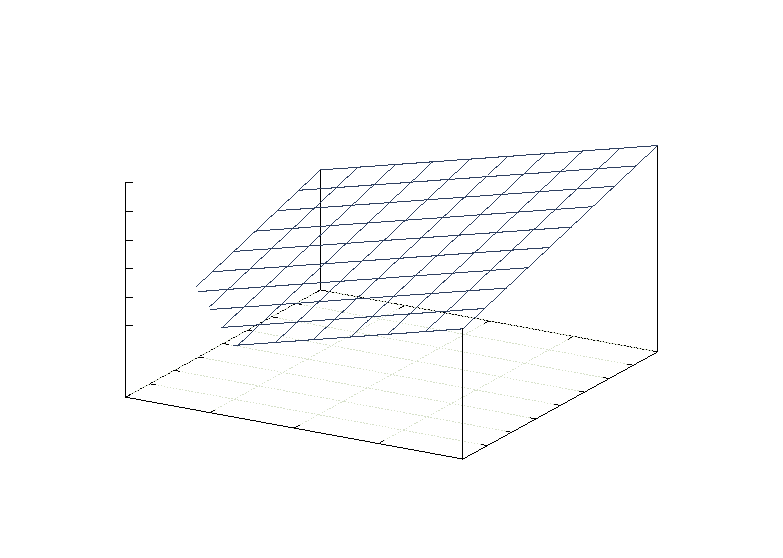
\includegraphics[trim=0 -0.51cm 0 0 ]{Graphs/2/Benchmark/Benchmark}}%
    \gplfronttext
  \end{picture}%
\endgroup
\hspace{2cm}}
			\caption[Energy benchmark model for a mining compressed air system]{Energy benchmark model for a mining compressed air system, adapted from Cilliers \cite{Cilliers2015PHD}}
			\label{fig: 3D Benchmark}
		\end{figure}
	%%%%%%%%%%%%%%%%%%%%%%%%%% Equation %%%%%%%%%%%%%%%%%%%%%%%%%%%%%
	%	\begin{equation}
	%	\label{eq: COLS}
	%	E_{comp} = 1.51\cdot Z + 33.36\cdot T - 1930.21
	%	\end{equation}			
	%%%%%%%%%%%%%%%%%%%%%%%%%%%%%%%%%%%%%%%%%%%%%%%%%%%%%%%%%%%%%%%%%%
	\subsection{Value of simulation in mining DSM}
	Van Niekerk \cite{van2013value},\cite{vanNiekerk2012Value} investigated the value of simulation models in mine \gls{dsm} projects. \cite{van2013value},\cite{vanNiekerk2012Value} developed simulation models for compressed air and water reticulation systems using KYPipes's gas simulation engine. 
	\par
	%\subsubsection{Mine cooling systems}
	Simulation has been used in studies as a tool to improve mine cooling. Holman \cite{Holman2014Masters} investigated improvements to mine cooling systems that improve performance and efficiency. In the study \cite{Holman2014Masters} used simplified \gls{ptb}  simulation models to investigate cooling interventions.
	\par 
	The scenario Holman simulated showed potential  average power reduction of 136 kW  which would lead to an annual energy cost saving of R0.55M. The study could be improved by increasing accuracy of the simulation. Power difference of as high as 31\% between the simulation and actual were observed for some time periods.
	\par
	%\subsubsection{Mine de-watering systems}	
	%\subsubsection{Mine compressed air systems}		
	Simulation has added great value for mining compressed air \gls{dsm}. A detailed literature discussion of compressed air simulation applications is discussed in Section  \ref{CompressorSimulation Literature}.
	\subsection{Simulation procedure}
	A structured simulation procedure is required to achieve the objectives of the study.  Previous studies from literature have focussed on how simulation software tools work rather the simulation procedure that was followed \cite{Mare2016PhD}.
	\par
	Bouwer \cite{bouwer2004designing} developed a software tool that he used to investigate large thermal and and energy. Bouwer used the following procedure to implement simulations:
	\begin{enumerate}
		\item Create a detailed schematic of the system
		\item Obtain data from installed instrumentation
		\item Perform manual measurements where necessary
		\item Gather data for a typical operational period
		\item Convert data into useful formats
		\item Set-up the simulation model
		\item Calibrate the model until simulated outputs match measured data
	\end{enumerate}
	Bouwer's simulation procedure provides a good guideline for mining system simulation. The procedure could be simplified by merging steps. For example step 1 to 4 could be merged into 1 step \enquote{Gather system data and information}.
	\subsubsection{Periodic/repeated simulation}
	The concept of periodic or repeated simulation procedure the execution a simulation multiple times or on a recurring schedule whilst altering various input parameters. \cite{Snyman2011Masters} used repeated estimation to determine an upper and lower bound for the expected result. Another example from industry is real time simulation or estimation systems.
	\par 
	 Van Heerden \textit{et al.} \cite{van2014developing} developed a dynamic control system for a mine compressed air network. The controller utilised repeated simulation to estimate unmeasured and future parameters of the network. This was used to optimise the compressor control.
	 \par
	Hollander and Lui \cite{Hollander2008Estimation} used repeated simulations to estimate travel time distributions for traffic networks. \cite{Hollander2008Estimation} developed the following methodology for the repeated simulations:
	\begin{enumerate}
		\item Gather input parameters
		\item Run simulations
		\item Read simulation outputs
		\item Repeat for desired iterations
	\end{enumerate}
\subsection{Available simulation tools}
A software tool is required to create and execute the compressed air simulations. In literature variety software tools have been used to simulate industrial systems. A suitable software system for this study must be capable of producing accurate models of complex compressed air network. The system should be able solve for transient compressed air simulation scenarios with dynamic data and control inputs. 
\par 
The development of system models should also not be excessively time-consuming. The software tools should also be able to handle missing data inputs and information that in common in mining systems.  These were shortfalls of simulation tools noted by van Tonder \cite{vanTonder2014PhD} and Marais \cite{Mare2016PhD}.
\par
The following simulation tools that may meet the criteria were identified : 
\begin{itemize}
	\item \gls{ptb}
	\item Flownex
	\item KYPipe GAS
	\item AirSim
	\item REMS
\end{itemize}
Of these tools, \gls{ptb} was identified as the most suitable software system for this study. Whilst it may be possible to use other packages, \gls{ptb} was developed specifically for simulation of mining systems. This allows simpler and speedier development of system components as many components such as compressor mathematical models have already been pre-built \cite{Mare2016PhD}. 
%\Gls{ptb}
%Mare \cite{Mare2016PhD} and Peach \cite{Peach2016Masters} investigated simulation software packages for mining systems; Identifying the strengths and limitations of each. 
 	\subsection{Simulation model verification strategies}\label{VerificationLit}
 	Due to lack of instrumentation, measurement inaccuracies and other non-ideal aspects of mining systems. It is impossible for a simulation model to match the actual system's performance perfectly. From literature, methods of verifying simulation precision were investigated. The verification techniques identified from literature were Mean residual difference, \gls{mae}, coefficient of determination or correlation and \gls{mse}.%Most studies utilised a comparison calculation strategy to calculate a model accuracy or error. %Two calculation methods identified were \emph{Average difference method} and \emph{average percentage difference}. 
 		\subsubsection{Mean residual difference method}
 			The average difference method looks at the average for the data points in the actual and simulated time series.  Relative error is then calculated with \cref{eq: AMean absolute}. The simulation percentage error in relation to the actual series is then calculated by dividing the error by the Actual data-points, \cref{eq: Average difference}.
 			
 			\begin{equation}
 			\label{eq: AMean absolute}
 			\bar{R} = \left| \dfrac{1}{N} \sum_{n=1}^{N}{ \left( A_{n} - S_{n}\right)}  \right|
 			\end{equation}
To get a relative error percentage, the equation is rewritten:	
 			\begin{equation}
 				\label{eq: Average difference}
 				Err_{\%} = \left| \dfrac{1}{N} \sum_{n=1}^{N}{ \left(\dfrac{ A_{n} - S_{n}}{A_n}\right)}  \right| \times 100 \%
 			\end{equation}
 			Where: \par 
 				\begin{table}[h!]
 					\centering
 					\begin{tabular}{cl}
 						$A$ & Actual system time series \\
 						$S$ & Simulation time series \\
 						$n$ & Data point \\
 						$N$ & Number of Data point in simulation period \\
 					\end{tabular} 
 				\end{table}	
 			A major disadvantage of this method is that for transient simulation, the positive and negative errors for individual points can cancel out. This leads to a smaller resultant error than would be expected. The resultant error therefore can not lead to any conclusive statements regarding the accuracy of the model \cite{sarin2010comparing}.  This strategy is not recommended if used alone to verify transient simulations. 
 			\par 
 						
 			Yu-jie Xu \textit{et al.} \cite{xu2016modeling} developed a steady state simulation of an absorption chiller. In the study \cite{xu2016modeling} utilised  residual difference to measure the relative steady state error of the absorber model. The accepted margin of accuracy in the study was a relative steady state error of 5\%. 
 			
 		\subsubsection{Mean absolute error method}
 		The \gls{mae} verification method follows a similar calculation as in the Average residual difference method. However, as shown in \cref{eq: Relative error}, the error is calculated individually for each point in the series. The average of the individually errors is the resultant error, \cref{eq: Relative error 2}. To obtain the relative error percentage, each error is divided by the Actual value at that time step as in \cref{eq: Relative error}.
 		\par
 		\begin{equation}
 		\label{eq: Relative error 2}
 		MAE = \dfrac{1}{N}\sum_{n=1}^{N}{\left|A_{n} - S_{n}\right| }
 		\end{equation}
 		
 			To get a relative error percentage, the equation is rewritten:	
 			\begin{equation}
 			\label{eq: Relative error}
 			Err_{\%} = \dfrac{1}{N}\sum_{n=1}^{N}{\left|\dfrac{A_{n} - S_{n}}{A_{n}}\right| }\times 100 \%
 			\end{equation}
 			Where: \par
 			\begin{table}[h!]
 				\centering
 				\begin{tabular}{cl}
 					$A$ & Actual system time series \\
 					$S$ & Simulation time series \\
 					$n$ & Data point \\
 					$N$ & Number of Data point in simulation period \\
 				\end{tabular} 
 			\end{table} 
 		\subsubsection{Coefficient of determination}
 		The Coefficient of correlation is the measure of how accurately a data series ($ x $) can be represented in a linear relationship with Data series ($ y $), i.e. $ y = mx+c$. The value for the coefficient ranges between $ -1 $ and $ 1 $ where a value of 1 indicates a perfect linear relationship between the series and a value of -1 represents a perfect negative linear relationship. A value of 0 indicate that there is no relationship between the data series. The correlation coefficient can be calculated using equation \cref{eq: Correlation coefficient}.\cite{sarin2010comparing}
 		
 		\begin{equation}
 		\label{eq: Correlation coefficient}
 		r = \dfrac{\sum_{n=1}^{N}(A_n - \bar{A})(S_n - \bar{S})}{\sqrt{\sum_{n=1}^{N}(A_n - \bar{A})^2 \cdot \sum_{n=1}^{N}(M_n - \bar{A})^2}}
 		\end{equation}
 		\par
 		Where \par
 		\begin{table}[h!]
 			\centering
 			\begin{tabular}{cl}
 				$A$ & Actual system time series \\
 				$S$ & Simulation time series \\
 				$n$ & Data point \\
 				$N$ & Number of Data point in simulation period \\
 			\end{tabular} 
 		\end{table}	
 		The coefficient of determination or R-Square value can be calculated by squaring the correlation coefficient (r). 
 		\par 
 			Kurnia \textit{et al} \cite{kurnia2014simulation},\cite{kurnia2014dust} developed a simulation for a novel underground mining ventilation system. \cite{kurnia2014simulation},\cite{kurnia2014dust} selected the mathematical model with the highest precision when compared with historical data points. The chosen model had an R-Square value of 0.96 and a relative error 30 \%, using the mean absolute error method. 
 			
 		\subsubsection{Mean squared error}	
 		In statistics, the \gls{mse} or \gls{rmse} is the average of the square of the error between the actual and estimated value. The value is always positive. A smaller value relates to a more accurate model.\footnote{University of Kentucky Department of Mathematics, "Estimators, Mean Square Error, and
 			Consistency" [Online] \url{http://www.ms.uky.edu/~mai/sta321/mse.pdf}, [Accessed 3 March 2017].}
 			\begin{equation}
 				\label{eq: rmse}
 				MSE = \dfrac{1}{N}\sum_{n=1}^{N}{(A_{n} - S_{n})^2}
 			\end{equation}
 			Where: \par
 			\begin{table}[h!]
 				\centering
 				\begin{tabular}{cl}
 					$A$ & Actual system time series \\
 					$S$ & Simulation time series \\
 					$n$ & Data point \\
 					$N$ & Number of Data point in simulation period \\
 			\end{tabular} 
 			\end{table}			
 		\subsubsection{Other methods}
 		A number of additional methods or variations of the methods discussed are available to verify transient simulations. As an example, \cite{arndt2007integrated} looked at the percentage of relative errors under a certain limits as well as a maximum relative error. The method is an improvement compared to residual  difference in ensuring transient simulation accuracy however the results are difficult to interpret.
 		\par
 		Sarin \textit{et al} \cite{sarin2010comparing} compared many methods. Some methods that have not been discussed in this study include:
 		\begin{itemize}
 			\item Vector Norms.
 			\item Sprague and Geers Metric \cite{Geers1984Objective},\cite{Sprague2004Spectral}
 			\item Russells error Measure \cite{Russell1},\cite{Russell2}
 			\item Normalized Integral Square Error
 			\item Dynamic Time Warping (DTW).
 		\end{itemize}
 		The calculations in the above methods are relatively complex. However, they provide additional metrics such as Phase, magnitude and slope errors. These metrics could add value in verifying simulations.
 		\subsubsection{Comparing verification methods}
 		The difference between the strategies is best shown using an example. Figure \cref{fig:Philipp Difference verify} shows the output and actual power of a simulation of a mining system for a 24 hour duration. In the study \cite{Mare2016PhD} used mean residual difference, \cref{eq: Average difference}, to determine the accuracy of a simulation model.
 		\par 
 		 Positive and negative differences between the simulated and actual profiles cancelled out, meaning the average value of the two power profiles were very similar. The calculated residual difference relative error was therefore calculated as 1.17\%. However, Using the relative error, \cref{eq: Relative error}, applied to the same data series results in a relative error of 15.2\%. The results of the verification strategies on the example is provided in \cref{Philip verification table}. 
 		
 	\begin{figure}[h!]
 		\centering
 		% GNUPLOT: LaTeX picture with Postscript
\begingroup
  \makeatletter
  \providecommand\color[2][]{%
    \GenericError{(gnuplot) \space\space\space\@spaces}{%
      Package color not loaded in conjunction with
      terminal option `colourtext'%
    }{See the gnuplot documentation for explanation.%
    }{Either use 'blacktext' in gnuplot or load the package
      color.sty in LaTeX.}%
    \renewcommand\color[2][]{}%
  }%
  \providecommand\includegraphics[2][]{%
    \GenericError{(gnuplot) \space\space\space\@spaces}{%
      Package graphicx or graphics not loaded%
    }{See the gnuplot documentation for explanation.%
    }{The gnuplot epslatex terminal needs graphicx.sty or graphics.sty.}%
    \renewcommand\includegraphics[2][]{}%
  }%
  \providecommand\rotatebox[2]{#2}%
  \@ifundefined{ifGPcolor}{%
    \newif\ifGPcolor
    \GPcolortrue
  }{}%
  \@ifundefined{ifGPblacktext}{%
    \newif\ifGPblacktext
    \GPblacktextfalse
  }{}%
  % define a \g@addto@macro without @ in the name:
  \let\gplgaddtomacro\g@addto@macro
  % define empty templates for all commands taking text:
  \gdef\gplbacktext{}%
  \gdef\gplfronttext{}%
  \makeatother
  \ifGPblacktext
    % no textcolor at all
    \def\colorrgb#1{}%
    \def\colorgray#1{}%
  \else
    % gray or color?
    \ifGPcolor
      \def\colorrgb#1{\color[rgb]{#1}}%
      \def\colorgray#1{\color[gray]{#1}}%
      \expandafter\def\csname LTw\endcsname{\color{white}}%
      \expandafter\def\csname LTb\endcsname{\color{black}}%
      \expandafter\def\csname LTa\endcsname{\color{black}}%
      \expandafter\def\csname LT0\endcsname{\color[rgb]{1,0,0}}%
      \expandafter\def\csname LT1\endcsname{\color[rgb]{0,1,0}}%
      \expandafter\def\csname LT2\endcsname{\color[rgb]{0,0,1}}%
      \expandafter\def\csname LT3\endcsname{\color[rgb]{1,0,1}}%
      \expandafter\def\csname LT4\endcsname{\color[rgb]{0,1,1}}%
      \expandafter\def\csname LT5\endcsname{\color[rgb]{1,1,0}}%
      \expandafter\def\csname LT6\endcsname{\color[rgb]{0,0,0}}%
      \expandafter\def\csname LT7\endcsname{\color[rgb]{1,0.3,0}}%
      \expandafter\def\csname LT8\endcsname{\color[rgb]{0.5,0.5,0.5}}%
    \else
      % gray
      \def\colorrgb#1{\color{black}}%
      \def\colorgray#1{\color[gray]{#1}}%
      \expandafter\def\csname LTw\endcsname{\color{white}}%
      \expandafter\def\csname LTb\endcsname{\color{black}}%
      \expandafter\def\csname LTa\endcsname{\color{black}}%
      \expandafter\def\csname LT0\endcsname{\color{black}}%
      \expandafter\def\csname LT1\endcsname{\color{black}}%
      \expandafter\def\csname LT2\endcsname{\color{black}}%
      \expandafter\def\csname LT3\endcsname{\color{black}}%
      \expandafter\def\csname LT4\endcsname{\color{black}}%
      \expandafter\def\csname LT5\endcsname{\color{black}}%
      \expandafter\def\csname LT6\endcsname{\color{black}}%
      \expandafter\def\csname LT7\endcsname{\color{black}}%
      \expandafter\def\csname LT8\endcsname{\color{black}}%
    \fi
  \fi
    \setlength{\unitlength}{0.0500bp}%
    \ifx\gptboxheight\undefined%
      \newlength{\gptboxheight}%
      \newlength{\gptboxwidth}%
      \newsavebox{\gptboxtext}%
    \fi%
    \setlength{\fboxrule}{0.5pt}%
    \setlength{\fboxsep}{1pt}%
\begin{picture}(9360.00,4536.00)%
    \gplgaddtomacro\gplbacktext{%
      \colorrgb{0.00,0.00,0.00}%
      \put(682,1584){\makebox(0,0)[r]{\strut{}$0$}}%
      \colorrgb{0.00,0.00,0.00}%
      \put(682,1853){\makebox(0,0)[r]{\strut{}$1$}}%
      \colorrgb{0.00,0.00,0.00}%
      \put(682,2121){\makebox(0,0)[r]{\strut{}$2$}}%
      \colorrgb{0.00,0.00,0.00}%
      \put(682,2390){\makebox(0,0)[r]{\strut{}$3$}}%
      \colorrgb{0.00,0.00,0.00}%
      \put(682,2659){\makebox(0,0)[r]{\strut{}$4$}}%
      \colorrgb{0.00,0.00,0.00}%
      \put(682,2927){\makebox(0,0)[r]{\strut{}$5$}}%
      \colorrgb{0.00,0.00,0.00}%
      \put(682,3196){\makebox(0,0)[r]{\strut{}$6$}}%
      \colorrgb{0.00,0.00,0.00}%
      \put(682,3465){\makebox(0,0)[r]{\strut{}$7$}}%
      \colorrgb{0.00,0.00,0.00}%
      \put(682,3734){\makebox(0,0)[r]{\strut{}$8$}}%
      \colorrgb{0.00,0.00,0.00}%
      \put(682,4002){\makebox(0,0)[r]{\strut{}$9$}}%
      \colorrgb{0.00,0.00,0.00}%
      \put(682,4271){\makebox(0,0)[r]{\strut{}$10$}}%
      \colorrgb{0.00,0.00,0.00}%
      \put(1286,1364){\makebox(0,0){\strut{}02:00}}%
      \colorrgb{0.00,0.00,0.00}%
      \put(1916,1364){\makebox(0,0){\strut{}04:00}}%
      \colorrgb{0.00,0.00,0.00}%
      \put(2546,1364){\makebox(0,0){\strut{}06:00}}%
      \colorrgb{0.00,0.00,0.00}%
      \put(3176,1364){\makebox(0,0){\strut{}08:00}}%
      \colorrgb{0.00,0.00,0.00}%
      \put(3805,1364){\makebox(0,0){\strut{}10:00}}%
      \colorrgb{0.00,0.00,0.00}%
      \put(4435,1364){\makebox(0,0){\strut{}12:00}}%
      \colorrgb{0.00,0.00,0.00}%
      \put(5065,1364){\makebox(0,0){\strut{}14:00}}%
      \colorrgb{0.00,0.00,0.00}%
      \put(5695,1364){\makebox(0,0){\strut{}16:00}}%
      \colorrgb{0.00,0.00,0.00}%
      \put(6325,1364){\makebox(0,0){\strut{}18:00}}%
      \colorrgb{0.00,0.00,0.00}%
      \put(6954,1364){\makebox(0,0){\strut{}20:00}}%
      \colorrgb{0.00,0.00,0.00}%
      \put(7584,1364){\makebox(0,0){\strut{}22:00}}%
      \colorrgb{0.00,0.00,0.00}%
      \put(8214,1364){\makebox(0,0){\strut{}00:00}}%
      \colorrgb{0.00,0.00,0.00}%
      \put(8346,1584){\makebox(0,0)[l]{\strut{}$0$}}%
      \colorrgb{0.00,0.00,0.00}%
      \put(8346,1853){\makebox(0,0)[l]{\strut{}$1$}}%
      \colorrgb{0.00,0.00,0.00}%
      \put(8346,2121){\makebox(0,0)[l]{\strut{}$2$}}%
      \colorrgb{0.00,0.00,0.00}%
      \put(8346,2390){\makebox(0,0)[l]{\strut{}$3$}}%
      \colorrgb{0.00,0.00,0.00}%
      \put(8346,2659){\makebox(0,0)[l]{\strut{}$4$}}%
      \colorrgb{0.00,0.00,0.00}%
      \put(8346,2927){\makebox(0,0)[l]{\strut{}$5$}}%
      \colorrgb{0.00,0.00,0.00}%
      \put(8346,3196){\makebox(0,0)[l]{\strut{}$6$}}%
      \colorrgb{0.00,0.00,0.00}%
      \put(8346,3465){\makebox(0,0)[l]{\strut{}$7$}}%
      \colorrgb{0.00,0.00,0.00}%
      \put(8346,3734){\makebox(0,0)[l]{\strut{}$8$}}%
      \colorrgb{0.00,0.00,0.00}%
      \put(8346,4002){\makebox(0,0)[l]{\strut{}$9$}}%
      \colorrgb{0.00,0.00,0.00}%
      \put(8346,4271){\makebox(0,0)[l]{\strut{}$10$}}%
      \csname LTb\endcsname%
      \put(1024,3000){\makebox(0,0)[l]{\strut{}\shortstack{Residual \\ difference}}}%
      \put(1024,1745){\makebox(0,0)[l]{\strut{}MAE}}%
      \put(1024,2014){\makebox(0,0)[l]{\strut{}MSE}}%
    }%
    \gplgaddtomacro\gplfronttext{%
      \csname LTb\endcsname%
      \put(176,2927){\rotatebox{-270}{\makebox(0,0){\strut{}Power $(MW)$}}}%
      \put(8851,2600){\rotatebox{-270}{\makebox(0,0){\strut{} Relative $Err_{\%} $}}}%
      \put(4514,1034){\makebox(0,0){\strut{}Time of use}}%
      \csname LTb\endcsname%
      \put(3659,833){\makebox(0,0)[r]{\strut{}AE \%}}%
      \csname LTb\endcsname%
      \put(3659,613){\makebox(0,0)[r]{\strut{}SE \%}}%
      \csname LTb\endcsname%
      \put(3659,393){\makebox(0,0)[r]{\strut{}MAE \%}}%
      \csname LTb\endcsname%
      \put(3659,173){\makebox(0,0)[r]{\strut{}MSE \%}}%
      \csname LTb\endcsname%
      \put(6890,833){\makebox(0,0)[r]{\strut{}Actual power}}%
      \csname LTb\endcsname%
      \put(6890,613){\makebox(0,0)[r]{\strut{}Simulated power}}%
      \csname LTb\endcsname%
      \put(6890,393){\makebox(0,0)[r]{\strut{}Average Actual}}%
      \csname LTb\endcsname%
      \put(6890,173){\makebox(0,0)[r]{\strut{}Average Simulation}}%
    }%
    \gplbacktext
    \put(0,0){\fbox{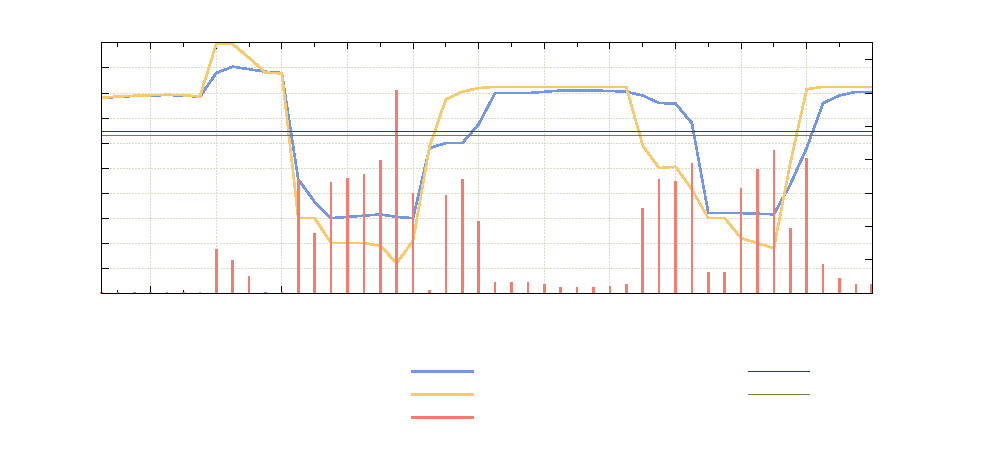
\includegraphics[trim=0 0 0.1cm 0, clip]{Graphs/2/Verification/Verification}}}%
    
    \gplfronttext
  \end{picture}%
\endgroup

 		\caption[Example of simulation error calculations.]{Example of simulation error calculations. Data adapted from Marè \cite{Mare2016PhD}}
 		\label{fig:Philipp Difference verify}
 	\end{figure}
 
 \begin{table}[h!]
 	\label{Philip verification table}
 	\centering
 	\begin{tabular}{lcr}
 		\hline
 		Verification method & Result & $Err_{\%}$\\
 		\hhline{===}
 		Residual Difference          & 0.06 MW difference  & 1.17\% \\
 		\gls{mae} 					 & 0.778 MW error & 15.2\% \\
 		\gls{mse} 				     & 1.236    & -\\
 		Coefficient of determination & $r^2 =0.857$   & -\\
 		\hline
 	\end{tabular} 
 \caption{Results of the comparison of verification methods.}
 \end{table}
 
 	\par 
 	Willmott \cite{willmott2005advantages} studied the Advantages of the use of mean absolute error \gls{mae} over the \gls{rmse} method in assessing model accuracy. In the study \cite{willmott2005advantages} concluded that the \gls{mse} measure is a function of \gls{mae} and therefore does not describe average error alone. From the analysis \gls{mae} was described as the most natural and unambiguous measure of average error magnitude.

 	\subsubsection{Verification usage in previous simulation studies}
 	Previous studies verified simulation accuracy through different methods and varying degrees of precision. \cref{table: Verification studies} summarises these approaches. The majority of local literature utilised the mean residual difference to determine the estimation accuracy. However, from literature it clear that the mean residual does not necessarily indicate model accuracy. \\
 	\begin{table}[h]
 		\centering
 		\begin{tabular}{p{5cm}ccr}
 			\hline
 			Study & Year & Verification method & Accepted margin\\
 			\hhline{====}
 			\shortstack{Arndt \cite{arndt2007integrated}\vspace{1em}}					& \shortstack{2000\vspace{1em}} & \shortstack{Mean and maximum\\ absolute \% error\vspace{0.5em}}  &\shortstack{ \% of time where \\ $Err_{\%} <10\%$ and\\ $Err_{\%} <5\%$ }\\
 			Bouwer \cite{bouwer2004designing}						& 2004 &Mean residual \% difference  & $Err_{\%} <10\%$ \\
 			Marais \cite{Marais2012PhD} 						& 2012 & Mean residual \% difference  & Not specified\\
 			Van Niekerk \cite{vanNiekerk2012Value} 				& 2012 &  Mean residual \% difference &  $Err_{\%} <10\%$  \\
 			Bredenkamp \cite{Bredenkamp2013Masters} 			& 2013 & Mean residual \% difference &  $Err_{\%} <10\%$  \\
 			Holman \cite{Holman2014Masters} 					& 2014 & Mean residual \% difference & Not specified  \\
 			Kriel \cite{Marais2012PhD} 							& 2014 &  Mean residual \% difference &  $Err_{\%} <10\%$  \\
 			VanTonder \cite{vanTonder2014PhD}					& 2014 &  Mean residual \% difference &  $Err_{\%} <3\%$  \\
 		\shortstack{Kurnia \textit{et al} \cite{kurnia2014simulation},\cite{kurnia2014dust} \vspace{0.25em}}	& \shortstack{2014\vspace{0.5em}} & \shortstack{Coefficient of determination \\Mean absolute error} & \shortstack{$r^2>0.95$ \\ $Err_{\%} <30\% $} \\ 
 			Dominic \cite{dominic2014dynamic}					& 2014 & Mean squared error & $<1.7e^{-3}$	\\
 			Du Plessis \textit{et al.}\cite{du2015development} 	& 2015 &  Mean residual \% difference &  $Err_{\%} <7\%$  \\
 			Pascoe \cite{Pascoe2016Masters} 					& 2016 &  Mean residual \% difference &  $Err_{\%} <5\%$  \\	
			Peach \cite{Peach2016Masters}						& 2016 &  Mean residual \% difference & Not specified\\
 			Mare \cite{Mare2016PhD} 							& 2016 &  Mean residual \% difference &  $Err_{\%} <5\%$   \\	
 			Yu-jie-Xu \textit{et al} \cite{xu2016modeling}		& 2016 &  Mean residual \% difference &  $Err_{\%} <5\%$ steady state \\
 			\hline
 		\end{tabular} 
 		\caption{Simulation verification methods that were implemented in previous studies.}
 		\label{table: Verification studies}
 	\end{table}
 	\subsection{Summary}
 	In this section the usage of simulation and estimation techniques to identify improvements in in mining industry was reviewed. Estimation and benchmark procedures in literature were first discussed. A review of simulation usage in mining DSM for water, compressed air and cooling systems was then discussed. 
 	\par 
 	Simulation procedures in literature were discussed. Various simulation software tools used in industry were than compared. Finally an analysis and comparison of verification procedures was performed.
 	
\section{Use of simulation in mining compressed air optimisation}
\label{CompressorSimulation Literature}
\subsection{Preamble}
This section will focus on discussion of literature regarding simulation usage in optimising mining compressed air systems. Shortcomings identified from literature that can be improved upon in this study will be addressed.
\subsection{Simplified compressed air simulation models} \label{simplfiedModels}
\subsubsection{Simplified "vessel"  model}
Before new software tools allowed for the development of detailed mining compressed air simulation models, Marais \cite{Marais2012PhD},\cite{marais2013simplification} created a simplified compressed air model to estimate and quantify the performance of potential energy interventions.  \cite{Marais2012PhD} simplified the mining compressed air system, comparing the network to an air source and a vessel with many leaks. This is illustrated in \cref{fig:Marais vessel model}.
\begin{figure}[h!]
	\centering
	\fbox{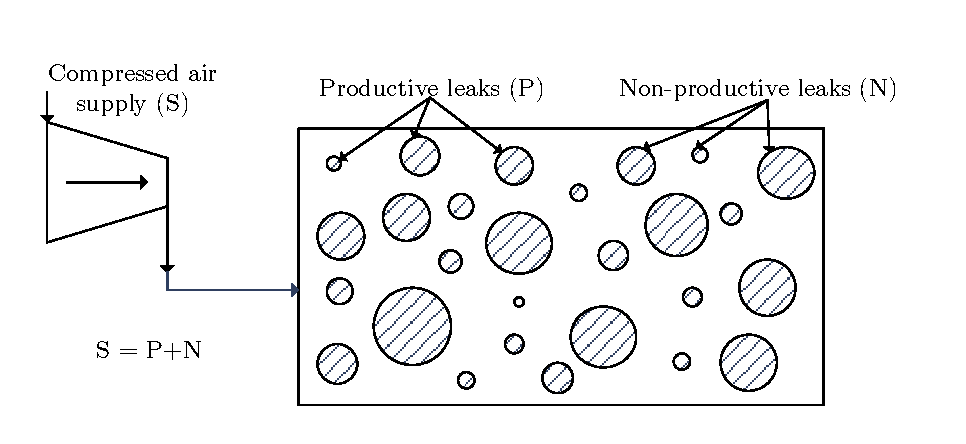
\includegraphics[width=\textwidth]{Images/2/marais/Vessel}}
	\caption[Simplified compressed air netowrk model.]{Simplified compressed air network model. Adapted from Marais \cite{Marais2012PhD}.}
	\label{fig:Marais vessel model}
\end{figure}
\par 
A simplified calculation methodology was developed to quickly estimate the expected energy savings impact on the system. From this, energy saving estimations rules were developed as listed in \cref{table: Rules of thumb}.  
\par 
\begin{table}[h]
	\centering
	\begin{tabular}{p{0.4\textwidth}p{0.05\textwidth}p{0.5\textwidth}}
		\hline
		Intervention && Estimation rule\\
		\hhline{===} 
		Reducing compressor deliver pressure & & $x \%$ pressure reduction  $\propto$ (1.6 to 1.8)$\cdot x\%$ power reduction \newline \\
		Reduce control valve pressure &  &$x \%$ pressure reduction $\propto$  $p\cdot x\%$ power reduction. \newline \newline Where p is the valves' relative flow contribution to the system \newline \\
		Reduction of flow && $x \%$ flow reduction  $\propto x \%$ power reduction \newline\\
		\hline
	\end{tabular} 
	\caption[Summary of energy saving estimation rules]{Summary of energy saving estimation rules\cite{Marais2012PhD}.}
	\label{table: Rules of thumb}
\end{table}
There is not a high degree of precision in this approach as specific details regarding the air network are not taken into account. The simplified approach cannot be used to estimate more complex scenarios. The method also does not estimate other potential benefits of interventions such as pressure delivery improvements.

\subsubsection{Simplified air network model}
Kriel \cite{Kriel2014Masters} used simulation to estimate the performance of energy projects on mining compressed air. The KYPipe GAS software tool was utilised to develop simulation models for the systems. \cite{Kriel2014Masters} simplified the air networks for the simulations to a single compressor representing the supply processes and an outlet flow to each underground level in the network. The model is shown graphically in \cref{fig:kriel  model}
\begin{figure}[h!]
	\centering
	\fbox{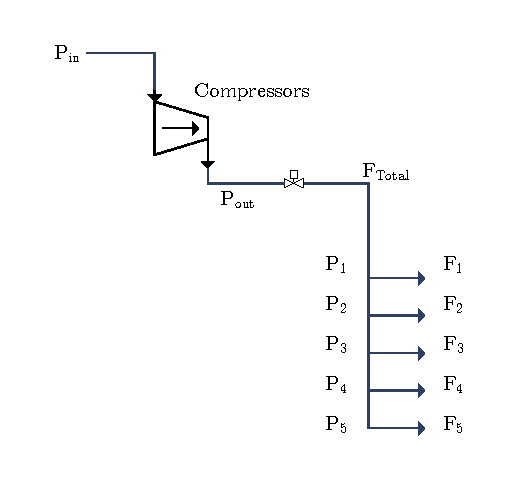
\includegraphics[trim =  -2cm 0.5cm -2cm 0.5cm ,width=\textwidth]{Images/2/kriel/model}}
	\caption[Simplified system model.]{Simplified system model. Adapted from Kriel \cite{Kriel2014Masters}.}
	\label{fig:kriel  model}
\end{figure}
\par 
Simulation was performed to quantify the savings from underground network interventions. The interventions were deigned to reduce flow to the network. The estimated savings from the simulations varied between 10 and 25\% compared to the actual performance of the interventions. Like the vessel model discussed previously, the simplified air network model can not be used to estimate the energy savings potential of more complex scenarios. The simulation procedure in this study could be improved by using a more detailed model and a more precise verification method. This would lead to savings predictions with higher accuracy. 

\subsection{Complex compressed air simulation models} \label{simplfiedModels}
\subsubsection{Compressor relocation}
Simulating compressor relocation requires air supply details that were neglected in the simplified simulation such models discussed in this section. Bredenkamp \cite{Bredenkamp2013Masters} therefore developed simulation models to test such compressor relocation scenarios. 
\par
The model takes into account the location, supply capacity of each compressor, as well as the surface pipe distances. The model, as visualised in \cref{fig: bredenkamp  model}, simplifies the air demand to an outlet flow per shaft.
\par
\begin{figure}[h!]
	\centering
	\fbox{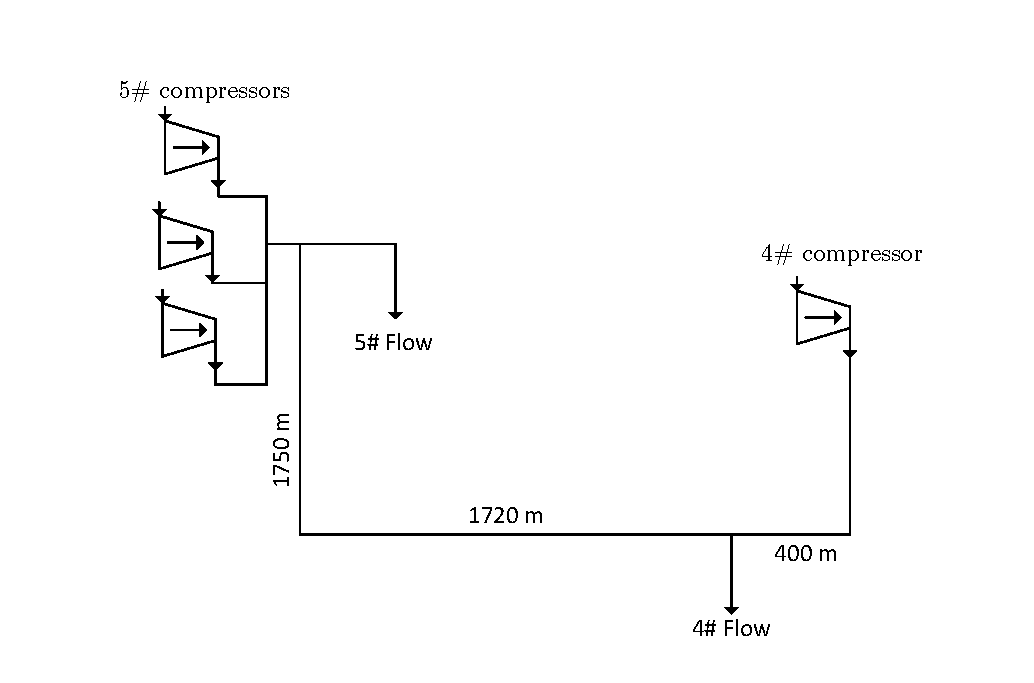
\includegraphics[trim =  -0.5cm 1cm -0.5cm 0cm ,width=\textwidth]{Images/2/bredenkamp/model}}
	\caption[Compressor relocation simulation model.]{Compressor relocation simulation model. Adapted from Bredenkamp \cite{Bredenkamp2013Masters}.}
	\label{fig: bredenkamp  model}
\end{figure} 
\cite{Bredenkamp2013Masters} utilised the residual difference to calibrate and verify the model parameters. Simulation precision and estimation confidence could therefore be improved through use of the other verification methods discussed in \cref{VerificationLit}.
\par 
Increasing the complexity of the demand components would provide more detailed results, showing more specific effects that result from the simulated scenarios.  Additionally more complex scenarios could be simulated with potentially greater savings

\subsubsection{Compressed air ring}
Pascoe \cite{Pascoe2016Masters} developed a simulation model for a compressed air ring. The purpose of the simulation was to identify the benefits of reducing pressure during the blasting shift period though valve control.\par 
 The model required complex supply side detail including modelling of individual compressor, locations of compressors and pipe lengths and control valves. The demand aspect of the system was simplified to a single flow per shaft, decline or processing plant. A schematic of the simulation model is shown in \cref{fig:Pascoe  model}.
 \par
\begin{figure}[h!]
	\centering
	\fbox{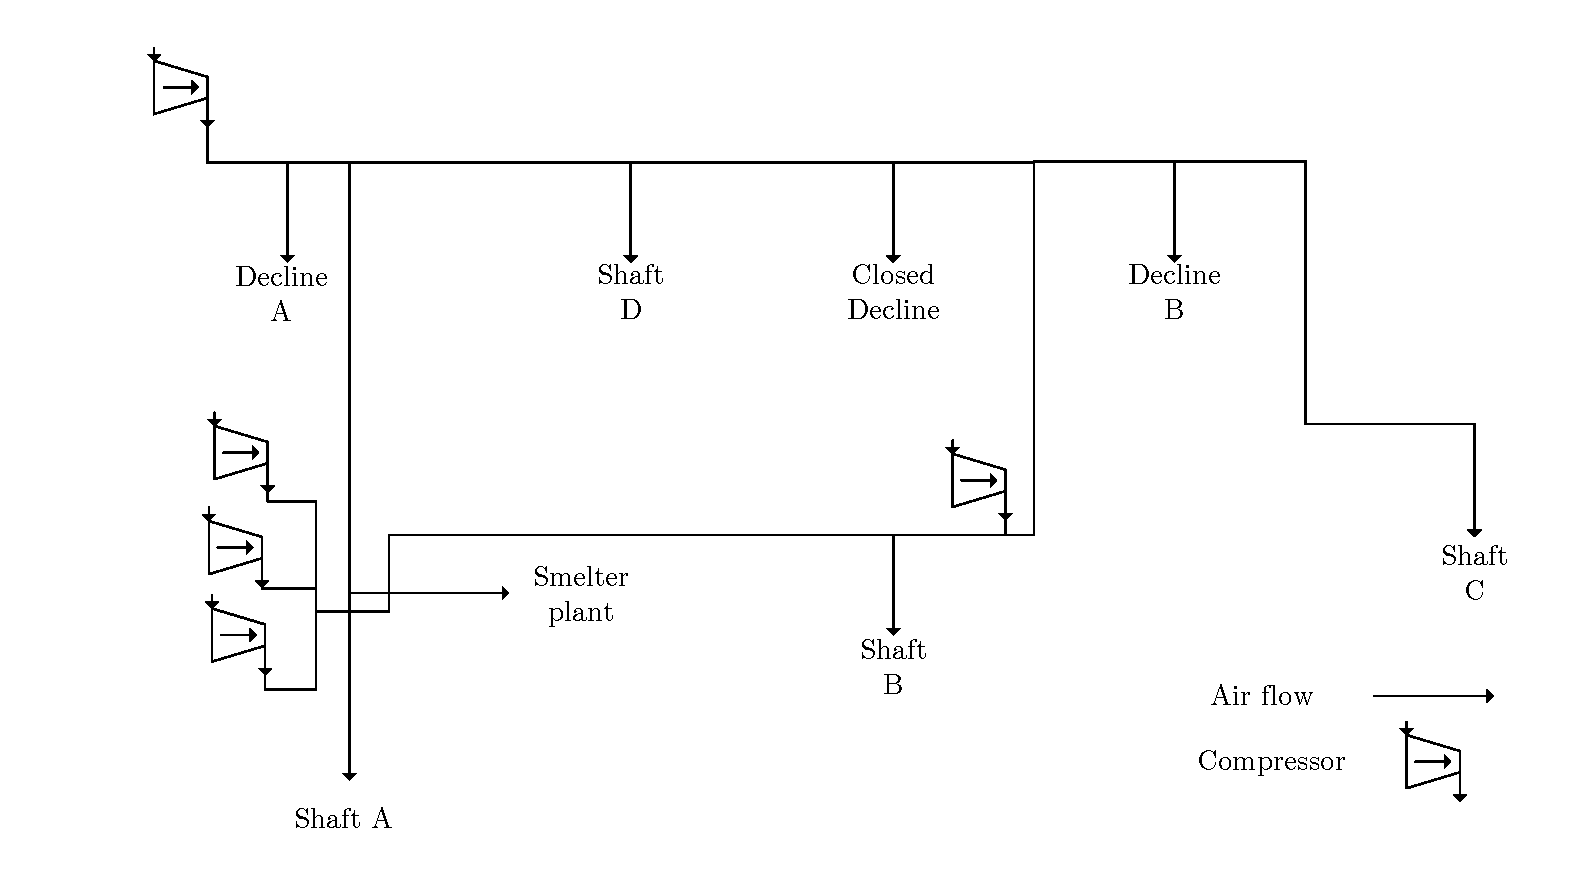
\includegraphics[trim =  -0.5cm 0.5cm -0.5cm 0.5cm ,width=\textwidth]{Images/2/pascoe/model}}
	\caption[Simplified compressed air ring model.]{Simplified compressed air ring model. Adapted from Pascoe \cite{Pascoe2016Masters}.}
	\label{fig:Pascoe  model}
\end{figure}
As was the case with Bredenkamp \cite{Bredenkamp2013Masters}, \cite{Pascoe2016Masters} utilised the residual difference to calibrate and verify the model parameters.The precision could therefore also be improved through the use of the other verification methods discussed in \cref{VerificationLit}. Increasing the complexity of the demand components could also be beneficial.

\subsubsection{Mine complex}
Maré \textit{et al.} \cite{Mare2017Evaluating} developed a compressed air simulation for a mining complex. In the study \cite{Mare2017Evaluating} simulated and prioritised several scenarios with the goal of reducing energy and other operational costs. 
\par
  Maré accurately modelled the individual compressors at each shaft in the mining complex. The detailed flow consumption at individual mining levels was found to be inaccurate. \cite{Mare2017Evaluating} therefore selected the process boundary for the model to include only the air flow consumption at the shaft. A process schematic for the simulation mode is shown in \cref{fig:Mare model}.
  
  \begin{figure}[h!]
  	\centering
  	\fbox{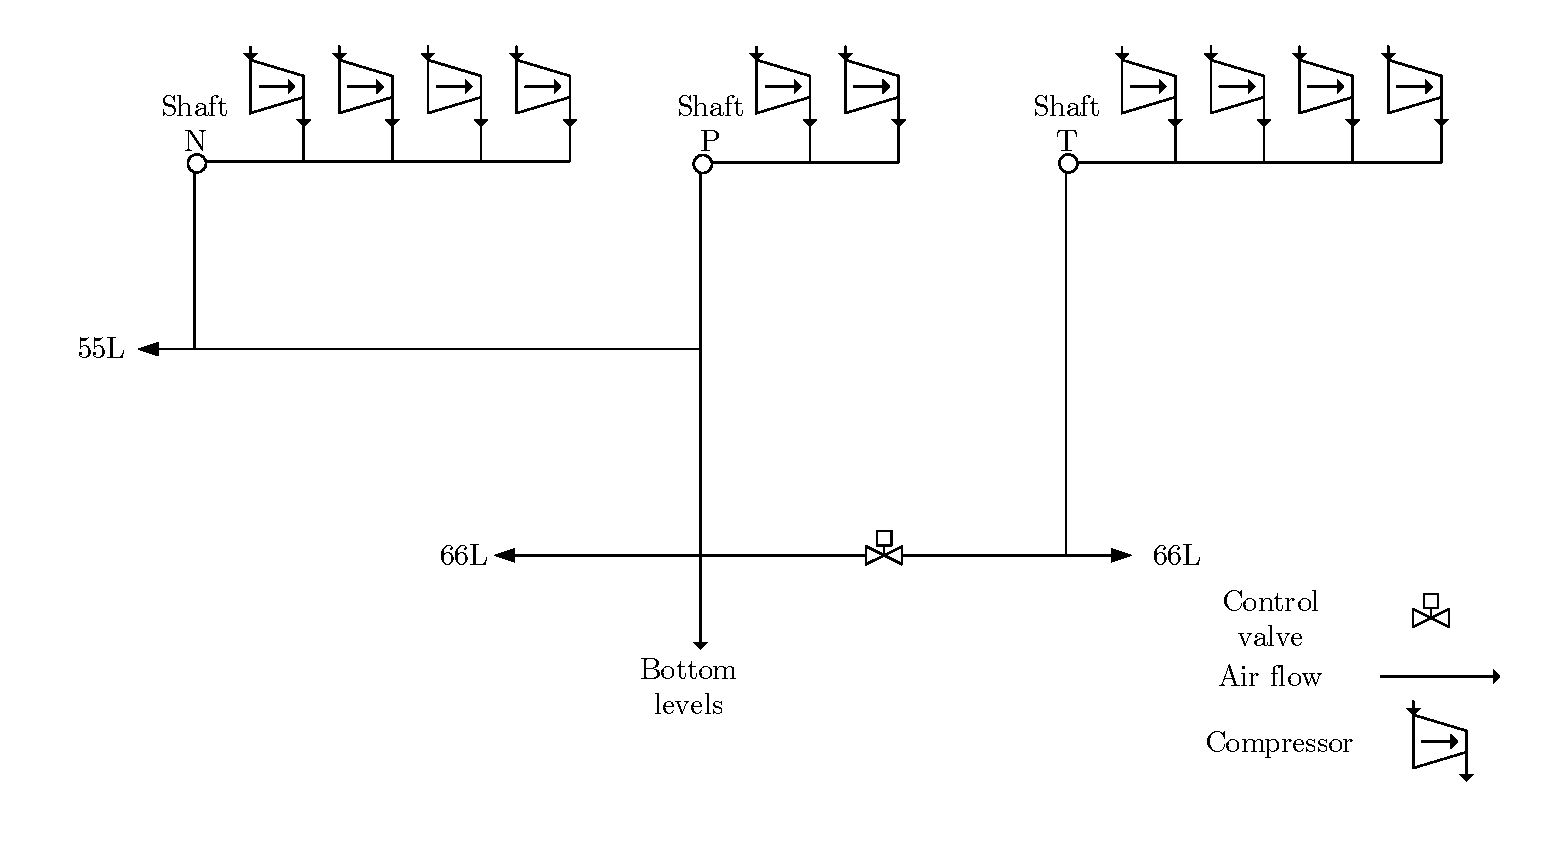
\includegraphics[trim =  -0.5cm 0.5cm -0.5cm 0.5cm ,width=\textwidth]{Images/2/mare/model}}
  	\caption[Simulation model for a complex air network.]{Simulation model for a complex air network. Adapted from Maré \textit{et al.} \cite{Mare2017Evaluating}.}
  	\label{fig:Mare model}
  \end{figure}
\par 
Using the model, 8 scenarios were simulated. The combined results showed that there was a potential energy saving of R1.5M as well as an additional pressure improvement of 51 kPa. The infrastructure and resource costs were estimated in order to prioritise the interventions for the greatest financial benefit to the mines.	
\par
	\cite{Mare2017Evaluating} used residual difference to calibrate and verify the accuracy of the transient simulations. Therefore The actual estimation error is therefore greater then what is shown in the study. Through on site inspections and strategic measurements, the detail of the simulation model could be improved this could allow for more accurate simulations and more simulation scenarios.
%- van Tonder\\
%- De Coning \\
	\subsection{Summary}\label{Shortcomings of previous work}
	Previous work in compressed air simulation was summarised and discussed in this section. Simplified and complex simulation models were discussed separately. Some of the shortcomings for simplified simulations was that they only provided generalised power saving results for the simulation.
	\par 
	The complex simulation models focussed on the details required for the scenarios that were simulated. Other aspects of the models were simplified as much as possible. This resulted in accurate, detailed results compared to the simplified models. However adding further complexity and detail could increase the the accuracy and allow for more simulation scenarios.
\section{Conclusion}
In Chapter 2, a comprehensive study of relevant literature was performed. the aim of the literature study was to :
\begin{itemize}
	\item Provide background on mining compressed air networks
	\item Review compressed air energy interventions in industry
	\item Review the usage of simulation in the mining industry industry
	\item Review the usage of simulation in the mining compressed air
\end{itemize}
Compressed air background was provided. This included background regarding various compressed air sub-components, the operational schedules and the effect on compressed air requirements  and finally the typical instrumentation found in a mining compressed air system.
\par
A review of previously achieved energy improvements in compressed air was the performed. The literature were divided into studies that focussed on improving the supply of compressed air and those that optimised the compressed air demand.
\par
The usage of simulation and estimation in mining industry was then reviewed. Estimation and benchmark procedures in literature were first discussed. this was followed by a review of simulation usage in mining DSM. Simulation procedures from literature were then discussed. Various simulation software tools used in industry were compared. Finally an analysis and comparison of verification procedures was performed.
\par 
	Finally, the usage of compressed air simulation was reviews. This included a discussion of simplified and complex simulation models. The shortcomings and success of previos studies were discussed.